\documentclass[compress]{beamer}

%--------------------------------------------------------------------------
% Common packages
%--------------------------------------------------------------------------
\usepackage[english]{babel}
\usepackage{pgfpages} % required for notes on second screen
\usepackage{graphicx}
\usepackage{subfigure}
\usepackage{multicol}
\usepackage[normalem]{ulem}

\usepackage{tabularx,ragged2e}
\usepackage{booktabs}
\usepackage{marvosym}

\makeatletter
\let\beamer@writeslidentry@miniframeson=\beamer@writeslidentry
\def\beamer@writeslidentry@miniframesoff{%
  \expandafter\beamer@ifempty\expandafter{\beamer@framestartpage}{}% does not happen normally
  {%else
    % removed \addtocontents commands
    \clearpage\beamer@notesactions%
  }
}
\newcommand*{\miniframeson}{\let\beamer@writeslidentry=\beamer@writeslidentry@miniframeson}
\newcommand*{\miniframesoff}{\let\beamer@writeslidentry=\beamer@writeslidentry@miniframesoff}
\makeatother


%--------------------------------------------------------------------------
% Load theme
%--------------------------------------------------------------------------
\usetheme{hri}

\usepackage{tikz}
\usetikzlibrary{patterns,shapes,fpu,fit,calc,mindmap,backgrounds,positioning,svg.path}

\tikzset{
  invisible/.style={opacity=0},
  visible on/.style={alt={#1{}{invisible}}},
  alt/.code args={<#1>#2#3}{%
    \alt<#1>{\pgfkeysalso{#2}}{\pgfkeysalso{#3}} % \pgfkeysalso doesn't change the path
  },
}


%%% great 'stop jumping' macro, to avoid tikz pictures to jump around when they
%%% change size in different overlays.
%%% usage: \tikzpicture[stop jumping]
% see: https://tex.stackexchange.com/a/51638
\newcounter{jumping}
\resetcounteronoverlays{jumping}

\makeatletter
\tikzset{
  stop jumping/.style={
    execute at end picture={%
      \stepcounter{jumping}%
      \immediate\write\pgfutil@auxout{%
        \noexpand\jump@setbb{\the\value{jumping}}{\noexpand\pgfpoint{\the\pgf@picminx}{\the\pgf@picminy}}{\noexpand\pgfpoint{\the\pgf@picmaxx}{\the\pgf@picmaxy}}
      },
      \csname jump@\the\value{jumping}@maxbb\endcsname
      \path (\the\pgf@x,\the\pgf@y);
      \csname jump@\the\value{jumping}@minbb\endcsname
      \path (\the\pgf@x,\the\pgf@y);
    },
  }
}
\def\jump@setbb#1#2#3{%
  \@ifundefined{jump@#1@maxbb}{%
    \expandafter\gdef\csname jump@#1@maxbb\endcsname{#3}%
  }{%
    \csname jump@#1@maxbb\endcsname
    \pgf@xa=\pgf@x
    \pgf@ya=\pgf@y
    #3
    \pgfmathsetlength\pgf@x{max(\pgf@x,\pgf@xa)}%
    \pgfmathsetlength\pgf@y{max(\pgf@y,\pgf@ya)}%
    \expandafter\xdef\csname jump@#1@maxbb\endcsname{\noexpand\pgfpoint{\the\pgf@x}{\the\pgf@y}}%
  }
  \@ifundefined{jump@#1@minbb}{%
    \expandafter\gdef\csname jump@#1@minbb\endcsname{#2}%
  }{%
    \csname jump@#1@minbb\endcsname
    \pgf@xa=\pgf@x
    \pgf@ya=\pgf@y
    #2
    \pgfmathsetlength\pgf@x{min(\pgf@x,\pgf@xa)}%
    \pgfmathsetlength\pgf@y{min(\pgf@y,\pgf@ya)}%
    \expandafter\xdef\csname jump@#1@minbb\endcsname{\noexpand\pgfpoint{\the\pgf@x}{\the\pgf@y}}%
  }
}
\makeatother


%% Neat trick to have only one navigation bullet per subsection
%% http://tex.stackexchange.com/questions/64333/one-navigation-bullet-per-subsection-with-subsection-false-in-custom-beamer-them
%\usepackage{etoolbox}
%\makeatletter
%\patchcmd{\slideentry}{\advance\beamer@xpos by1\relax}{}{}{}
%\def\beamer@subsectionentry#1#2#3#4#5{\advance\beamer@xpos by1\relax}%
%\makeatother
%%%%%%%%%%%%%%%%%%%%%%%%%%%%%%%%%%%%%%%

\graphicspath{{figs/}}

% for model of anthopomorphism
\newcommand{\IPA}{{$\mathcal{A}_0$~}}
\newcommand{\SLA}{{$\mathcal{A}_\infty$~}}
\newcommand{\sla}{{\mathcal{A}_\infty}}
\newcommand{\AntMax}{{$\mathcal{A}_{max}$~}}
\newcommand{\antMax}{{\mathcal{A}_{max}}}

% for HATP plans
\newcommand{\hatpaction}[3]{#1\\\textsf{\scriptsize #2,}\\\textsf{\scriptsize #3}}
\newcommand{\stmt}[1]{{\footnotesize \tt  #1}}

% for mutual modelling
\newcommand{\Mmodel}[3]{{\mathcal{M}(#1, #2, #3)}}
\newcommand{\model}[3]{{$\mathcal{M}(#1, #2, #3)$}}
\newcommand{\Model}[3]{{$\mathcal{M}^{\circ}(#1, #2, #3)$}}

% typeset logical concept
\newcommand{\concept}[1]{{\scriptsize \texttt{#1}}}

\newcommand{\backbutton}{\hfill\hyperlink{appendix}{\beamerreturnbutton{Supplementary material}}}
%--------------------------------------------------------------------------
% General presentation settings
%--------------------------------------------------------------------------
\title{child-robot interaction for learning}
\subtitle{are we ready yet to push the classroom's door?}
\date{{\bf  Robot4SEN} -- 05 Jul. 2019}
\author{Séverin Lemaignan}
\institute{{\bf Bristol Robotics Lab} University of the West of England}

%--------------------------------------------------------------------------
% Notes settings
%--------------------------------------------------------------------------
%\setbeameroption{show notes on second screen}
%\setbeameroption{hide notes}

\begin{document}


%%%%%%%%%%%%%%%%%%%%%%%%%%%%%%%%%%%%%%%%%%%%%%%%%%%%%%%%


%%%%%%%%%%%%%%%%%%%%%%%%%%%%%%%%%%%%%%%%%%%%%%%%%%%%%%%%

\maketitle

\licenseframe{github.com/severin-lemaignan/child-robot-interaction-for-learning}

\videoframe[0.56]{figs/cowriter/nao-tablet-demo.mp4?autostart}

\begin{frame}[plain]

    Quick poll:
    
    \begin{center}
        \Large {\bf
    What is the greatest challenge that ``child-robot interaction
        for learning'' faces today?}
    \end{center}

    \pause

    Lack of appropriate teaching material?

    \pause

    Getting robots accepted \& used in schools, without engineers/researchers
    being around...?

\end{frame}

\imageframe[color=black]{paul_experimental_setup}
\imageframe[color=black]{ranger-side}

% how engineers/researchers see the problem
\imageframe[color=black,caption={open, underspecified situations\par
complex~social~dynamics\par rich~semantics\par
interplay~of~socio-cognitive~functions\par
(and~ideally,~a~bit~of~actual~learning)}]{robots-classroom}

% how teachers/schools see the problem -> practical approach!
\imageframe[color=black]{robot4SEN/collage}

\imageframe[color=black,caption=Let's frame it bit]{robots-classroom}
\imageframe[color=black]{cri-focus-child-robot}
\imageframe[color=black]{cri-focus-child-robot-teacher}
\imageframe[color=black]{robots-classroom}

\imageframe[color=black]{interactions-actors}
\imageframe{interactions-cr}
\imageframe{interactions-crt}
\imageframe{interactions-ccrt}
\imageframe{interactions-ccrtg}
\imageframe{interactions-ccrtgc}


%\section{What challenges are we talking about, exactly?}
%
%{
%\paper{Baxter, Lemaignan, Trafton {\bf Workshop on Cognitive Architectures for Social HRI} -- HRI 2016}
%\begin{frame}<5>{Surface functions for Social Cognition}
%\centering
%        \resizebox{!}{0.7\paperheight}{%
%            \begin{tikzpicture}[
%                    >=latex,
%                every edge/.style={<-, draw, very thick}]
%        
%
%            \path[small mindmap, 
%                level 1 concept/.append style={sibling angle=360/6}, 
%                level 2 concept/.append style={sibling angle=60}, 
%            concept color=white,text=hriWarmGreyDark]
%            node[concept, visible on=<1-5>] {\bf Social\\Cognition in HRI}
%            [clockwise from=30]
%            child[concept color=hriSec1,text=white] { node[concept] (percept) {Perception of Human's State}
%                [clockwise from=120]
%                child[concept color=hriSec3Dark,text=white] { node[concept]
%                (emotions) {Empathy Emotions} }
%                child[concept color=hriSec2Dark,text=white] { node[concept] (attention) {Attention} }
%                child[concept color=hriSec2CompDark,text=white] { node[concept] (mmodel) {Inference of mental models} };
%            }
%            child[concept color=hriSec2Comp,text=white,grow=-45, visible on=<2->] { node[concept] (knowledge) {Social Knowledge} 
%                [counterclockwise from=-140]
%                child[concept color=hriSec1CompDark,text=white] { node[concept] (soc-rules) {Social rules} }
%                child[concept color=hriSec3Comp,text=black] { node[concept] (soc-ctxt) {Social context} }
%                child[concept color=hriSec2Dark,text=white] { node[concept] (memory) {Social memory} }
%                child[concept color=hriSec3CompDark,text=white] { node[concept] (common-sense) {Common-sense} };
%            }
%            child[concept color=hriSec3Comp,text=black, grow=-120,visible on=<3->] { node[concept] (comm) {Communication} 
%                [counterclockwise from=180]
%                child[concept color=hriSec1CompDark,text=white] { node[concept] (dialog) {Verbal} }
%                child[concept color=hriSec1Dark,text=white] { node[concept] (non-verbal) {Non-verbal} };
%            }
%            child[concept color=hriSec3,text=white,grow=180,visible on=<4->] { node[concept] (dynamics) {Interaction Dynamics} 
%                [clockwise from=180]
%                child[concept color=hriSec2Dark,text=white] { node[concept] (long-term) {Long-term interaction} };
%            }
%            child[concept color=hriSec2,text=black, grow=120,visible on=<5->] { node[concept] (action) {Performing with humans} 
%                [counterclockwise from=80]
%                child[concept color=hriSec2CompDark,text=white] { node[concept] {Action, behaviour recognition} }
%                child[concept color=hriSec1Dark,text=white] { node[concept] {Intention reading} }
%                child[concept color=hriSec3,text=white] { node[concept] (joint-action) {Joint actions} };
%            };
%
%
%        \end{tikzpicture}
%    }
%    \badge{plym}
%\end{frame}
%}


\section{The classroom}

 \begin{frame}[plain]
     
        \Large
     What is the most effective learning tool in a classroom?
 \end{frame}

%%%%%%%%%%%%%%%%%%%%%%%%%%%%%%%%%%%%%%%%%%%%%%%%%%%%%%%%


 \imageframe[color=black]{cellulo/pencil}

 \begin{frame}{Why that?}

     \begin{itemize}
         \item<1-> {\bf ubiquitous}: a pervasive yet unremarkable tool
             that blend into the daily learning routine; has to be
             trustworthy(\ie reliable), readily replaceable (\ie cheap, no
             affective bonding), intuitive (\ie few simple affordances)

         \item<2-> {\bf versatile}: applicable to a broad range of learning
             scenarios; good tools are not overly specialised (appearance and
             interaction modalities do not imply or force a specific/unique use
             case)

         \item<3-> {\bf effective}: to gain broad
             acceptance in a classroom, a tool must critically
             represent a net educative gain and must not incur higher
             workload for the teacher
     \end{itemize}
 \end{frame}


 \imageframe[caption=Pens and paper are pervasive...]{cellulo/classroom}
 \imageframe[caption=...what about robots?]{cellulo/classroom}

\imageframe[color=black]{robot4SEN/pano.jpg}

\begin{frame}[plain]
    \Large\bf\centering
    What does it take to build a pen-like robot?
\end{frame}

%%%%%%%%%%%%%%%%%%%%%%%%%%%%%%%%%%%%%%%%%%%%%%%%%%%%%%%%
%%%%%%%%%%%%%%%%%%%%%%%%%%%%%%%%%%%%%%%%%%%%%%%%%%%%%%%%


%%%%%%%%%%%%%%%%%%%%%%%%%%%%%%%%%%%%%%%%%%%%%%%%%%%%%%%%

{
    \paper{\"Ozg\"ur, Lemaignan et al. {\bf Cellulo: Versatile Handheld Robots
    for Education} -- HRI 2017}
 \begin{frame}{Design principles for the classroom}

     \begin{itemize}
         \item<1-> {\bf ubiquitous}: a pervasive yet unremarkable tool
             that blend into the daily learning routine; has to be
             trustworthy(\ie reliable), readily replaceable (\ie cheap, no
             affective bonding), intuitive (\ie few simple affordances)

         \item<2-> {\bf versatile}: applicable to a broad range of learning
             scenarios; the robots’ hardware, appearance and interaction
             modalities must not imply or be constrained to specific use cases

         \item<3-> {\bf effective}: to gain field
             acceptance in the classrooms, educative robots must critically
             represent a net educative gain and must not incur higher
             workload for the teachers (\textbf{easy orchestration})
     \end{itemize}

 \end{frame}
}

\imageframe{cellulo/classroom}
\imageframe{cellulo/classroom-withcellulo}

%%%%%%%%%%%%%%%%%%%%%%%%%%%%%%%%%%%%%%%%%%%%%%%%%%%%%%%%

 \begin{frame}{Cellulo: hardware}
     \begin{center}
         
\includegraphics[width=0.8\linewidth]{cellulo/hardware-design}
     \end{center}
     \begin{itemize}
         \item Holonomic motion
         \item Sub-mm absolute localisation (no external hardware)
         \item Haptic feedback + tactile RGB LED buttons 
         \item Bluetooth
         \item<2> Affordable (prototype: \EUR125)
     \end{itemize}
        \badge{ayberk-epfl}
 \end{frame}

%%%%%%%%%%%%%%%%%%%%%%%%%%%%%%%%%%%%%%%%%%%%%%%%%%%%%%%%

 \videoframe[0.56]{figs/cellulo/cellulo-swarm-demo.mp4}

%%%%%%%%%%%%%%%%%%%%%%%%%%%%%%%%%%%%%%%%%%%%%%%%%%%%%%%%
%%%%%%%%%%%%%%%%%%%%%%%%%%%%%%%%%%%%%%%%%%%%%%%%%%%%%%%%

 \imageframe[color=black,caption=Concept 1: chemistry]{cellulo/concept-molecules}

%%%%%%%%%%%%%%%%%%%%%%%%%%%%%%%%%%%%%%%%%%%%%%%%%%%%%%%%

 \imageframe[color=black,caption=Concept 2: solar system]{cellulo/concept-solar-system}


 \videoframe[0.56]{figs/cellulo/rehab.mp4?start=32&stop=74}

%%%%%%%%%%%%%%%%%%%%%%%%%%%%%%%%%%%%%%%%%%%%%%%%%%%%%%%%
%
%{
%    \paper{\"Ozg\"ur, Lemaignan et al. {\bf Cellulo: Versatile Handheld Robots
%    for Education} -- HRI 2017}
% \begin{frame}{Interaction Design space}
%     \begin{center}
%         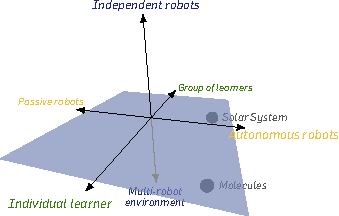
\includegraphics[width=0.8\linewidth]{cellulo/interaction-space}
%     \end{center}
%        \badge{ayberk-epfl}
% \end{frame}
% }
%
%%%%%%%%%%%%%%%%%%%%%%%%%%%%%%%%%%%%%%%%%%%%%%%%%%%%%%%%

 \begin{frame}[plain]{}

     \centering
    If a ``pen-like'' robot is actually doable,


     \Large\bf
     ...are social robots relevant at all...?
 \end{frame}

 \imageframe[color=black, caption={Yes, maybe...!}]{cowriter/social-learning}
%
%\begin{frame}[label=cowriter-impl]{Technical Challenges}
%    \badge{epfl}
%    \begin{itemize}
%        \item<1-> Get a child-proof robot to write...
%        \item<2-> ...badly...
%        \item<3-> Make it able to learn...
%        \item<4-> ...with the help of children
%    \end{itemize}
%\end{frame}

\section{The teacher}


{
    \fullbackground[scale=0.9]{sparc/sparc-bg}
\begin{frame}[plain]
    \Large
    Beyond the question of the practical integration of robots into the
    classroom, how to address \textbf{teachers' acceptance}, and specifically, the \textbf{tension between robot autonomy and teacher
    control}?

\end{frame}
}

%\imageframe[caption={\textbf{Interactive Reinforcement Learning} to the rescue?}, color=black]{sparc/sophies}

\begin{frame}{Autonomous robot, yet teacher in the loop?}

    One experiment with:
    
    \begin{itemize}
        \item<+-> a real robot
        \item<+-> a real interaction (...with a human!)
        \item<+-> a continuous interaction
        \item<+-> a realistic task (large state vector \& action space)
        \item<+-> also including social behaviours \& social dynamics
    \end{itemize}

    \badge{emmanuel}
\end{frame}

\imageframe[color=black,caption={$|state| = 210$ $| action\_space| = 655$}]{sparc/gui}
\imageframe[color=black]{sparc/overview}
\videoframe[0.56]{figs/sparc/video.mp4}
%\imageframe[color=black]{sparc/woz-gui}
%\imageframe[caption={Overall performance (pre-, mid-, post-test)},scale=0.9]{sparc/perf}
\imageframe[scale=0.9]{sparc/actions-supervised}
\imageframe[scale=0.9]{sparc/actions}
\imageframe[scale=0.9]{sparc/social-timing}

\begin{frame}{What does that means for the teacher?}

    \begin{columns}
        \begin{column}{0.45\linewidth}
            
            \begin{center}
                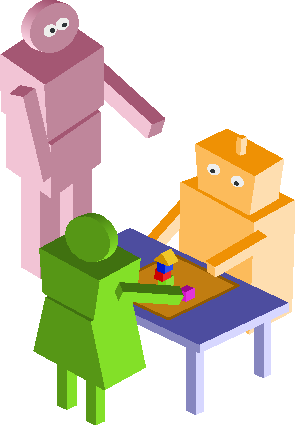
\includegraphics[width=0.9\linewidth]{sparc/sparc}
            \end{center}
        \end{column}
        \begin{column}{0.55\linewidth}
            \only<1>{
            \begin{itemize}
                \item {\bf Progressively transferring autonomy}  demonstrably
                    works in non-trivial tutoring scenarios

                \item (it also learns some elements of {\bf social behaviours} and
                    {\bf social timing})
            \end{itemize}
        }
            \only<2>{
                Key properties:

            \begin{itemize}
                \item \textbf{progressive autonomy} yet
                    \textbf{transparency} of the behaviour;
                \item \textbf{observability} and possibility to \textbf{take
                    over};
                \item because the training takes place in-situ, the
                    robot behaviours are \textbf{co-constructed} by the
                    teacher and the child
            \end{itemize}
        }
            \only<3>{
                Yet:

            \begin{itemize}
                \item Design of the input state tricky and largely task
                    dependent;
                \item What about more complex social behaviours?
                \item Nothing yet on group dynamics
            \end{itemize}
            }
        \end{column}
    \end{columns}


\end{frame}

%%%%%%%%%%%%%%%%%%%%%%%%%%%%%%%%%%%%%%%%%%%%%%%%%%%%%%%%
%%%%%%%%%%%%%%%%%%%%%%%%%%%%%%%%%%%%%%%%%%%%%%%%%%%%%%%%

\section[The children]{The children: the challenge of ``doing together''}
%%%%%%%%%%%%%%%%%%%%%%%%%%%%%%%%%%%%%%%%%%%%%%%%%%%%%%%%

\begin{frame}{Social or not Social?}
     \begin{center}
         \resizebox{\linewidth}{!}{
             \begin{tikzpicture}[>=latex]
                 \node[double arrow,draw] (spec) {Interaction spectrum};
                 \node<1>[minimum size=3cm,left=of spec] {Non-social};
                 \node<2>[minimum size=3cm,left=of spec] {Tool?};
                 %\node<3>[minimum size=3cm,left=of spec] {\bf Cellulo};
                 \node<1>[minimum size=3cm,right=of spec] {Social};
                 \node<2>[minimum size=3cm,right=of spec] {Peer/tutor?};
                 %\node<3>[minimum size=3cm,right=of spec] {\bf CoWriter};
             \end{tikzpicture}
         }
     \end{center}
\end{frame}


%%%%%%%%%%%%%%%%%%%%%%%%%%%%%%%%%%%%%%%%%%%%%%%%%%%%%%%%

\imageframe[color=black]{cowriter/diego-writing}

{
    \paper{Lemaignan et al. {\bf Learning by Teaching a Robot: The Case of Handwriting} -- Robotics and Automation Magazine 2016}

\begin{frame}{The CoWriter project}
    \badge{epfl}

    Can we address children' hand-writing impairments with robots?

    \begin{itemize}
        \item<2-> Robots do not know how to write!
        \item<3-> Learning by Teaching
        \item<4-> (nice side-effect: we can adapt to each child and each disabilities)
    \end{itemize}
\end{frame}
}

\videoframe[0.56]{figs/cowriter/training-s.mp4?autostart&noaudio}

{
    \paper{Hood, Lemaignan et al. {\bf When Children Teach a Robot to Write: An
    Autonomous Teachable Humanoid [...]} -- HRI 2015}

\begin{frame}{Learning from demonstration}
    \begin{center}
    
\includegraphics[width=0.8\textwidth]{cowriter/learningSdemo.png}
    \end{center}
    \badge{deana-epfl}
\end{frame}

}


\imageframe[color=black]{cowriter/diego-correct}

\begin{frame}{Before -- After}
    \begin{center}
        \only<1-2>{
        \includegraphics[width=0.43\linewidth]{cowriter/lettre-base}
        \uncover<2>{
            \hspace{1cm}%
        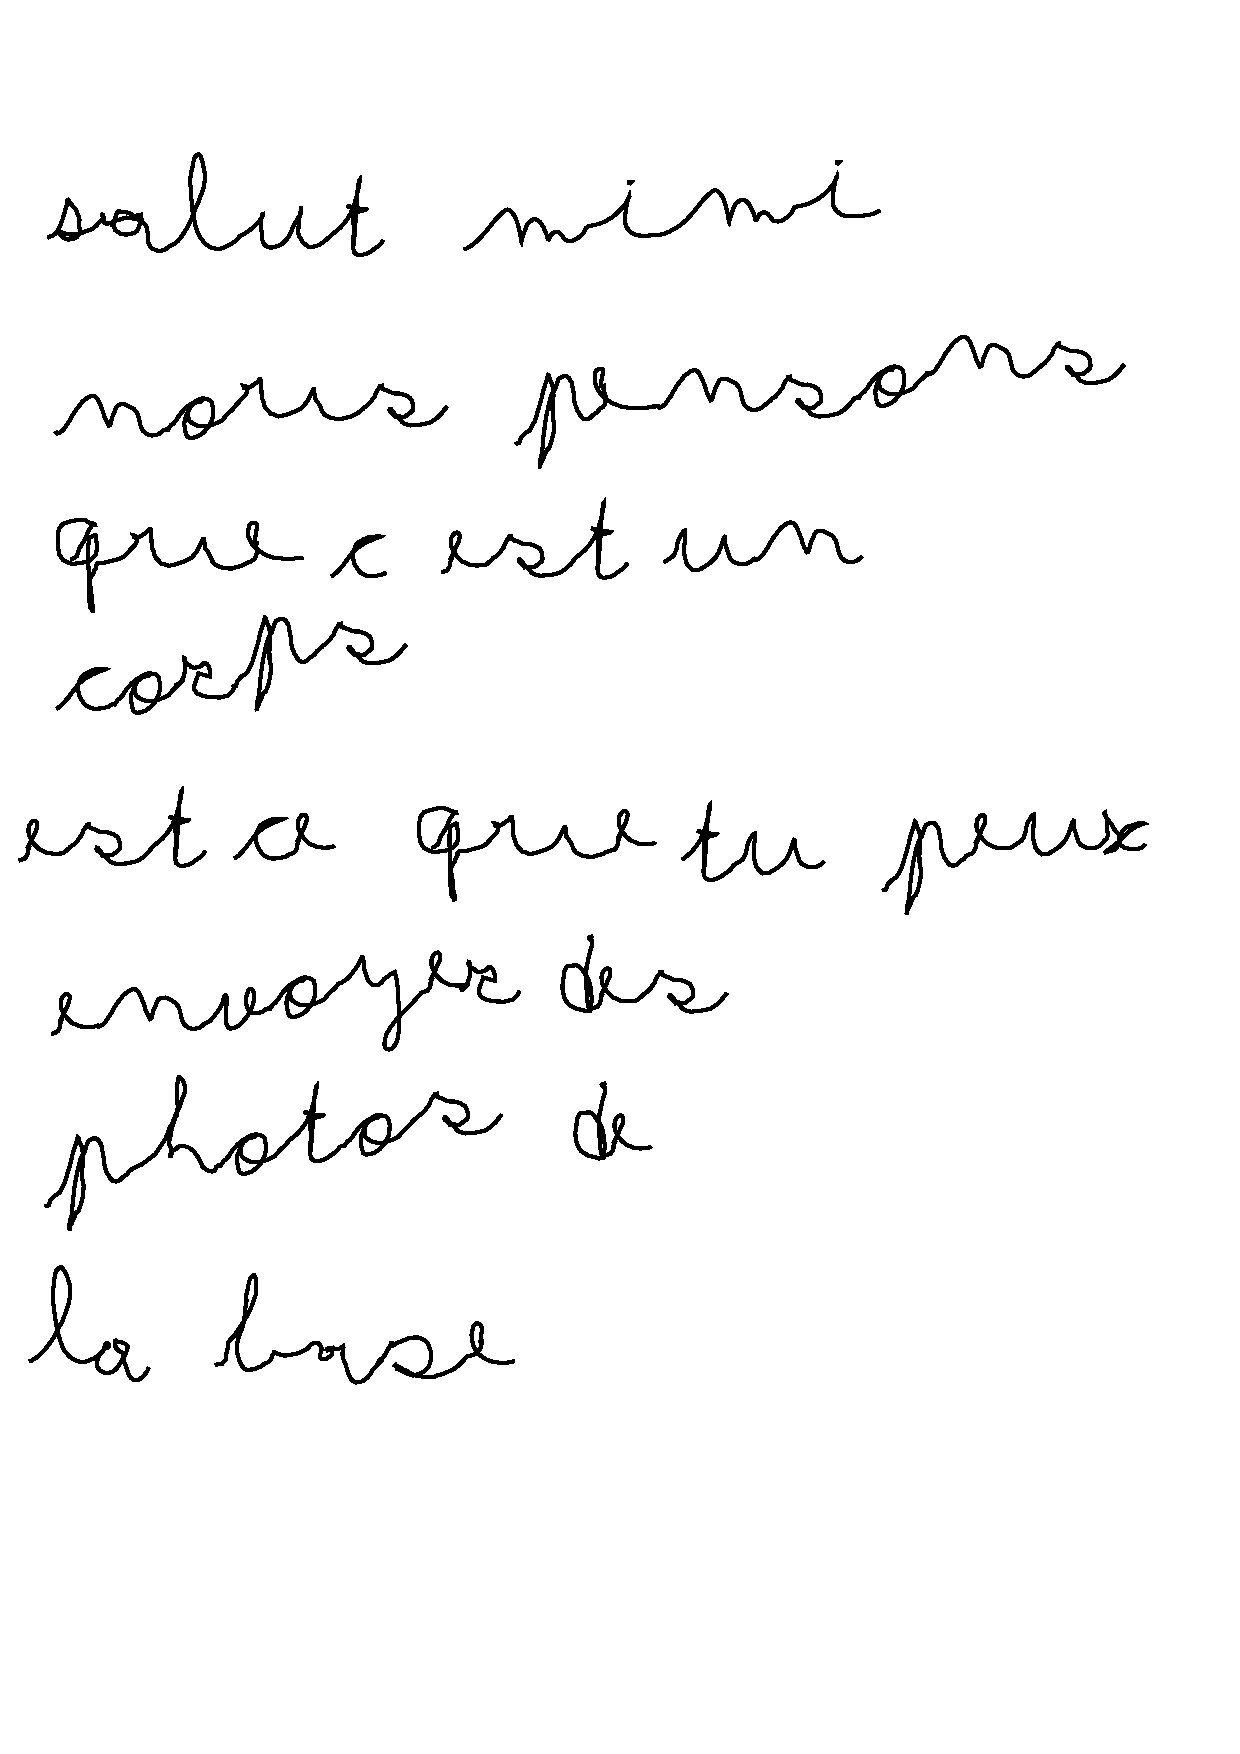
\includegraphics[width=0.43\linewidth]{cowriter/lettre-final}
        }
        }
        \only<3>{
        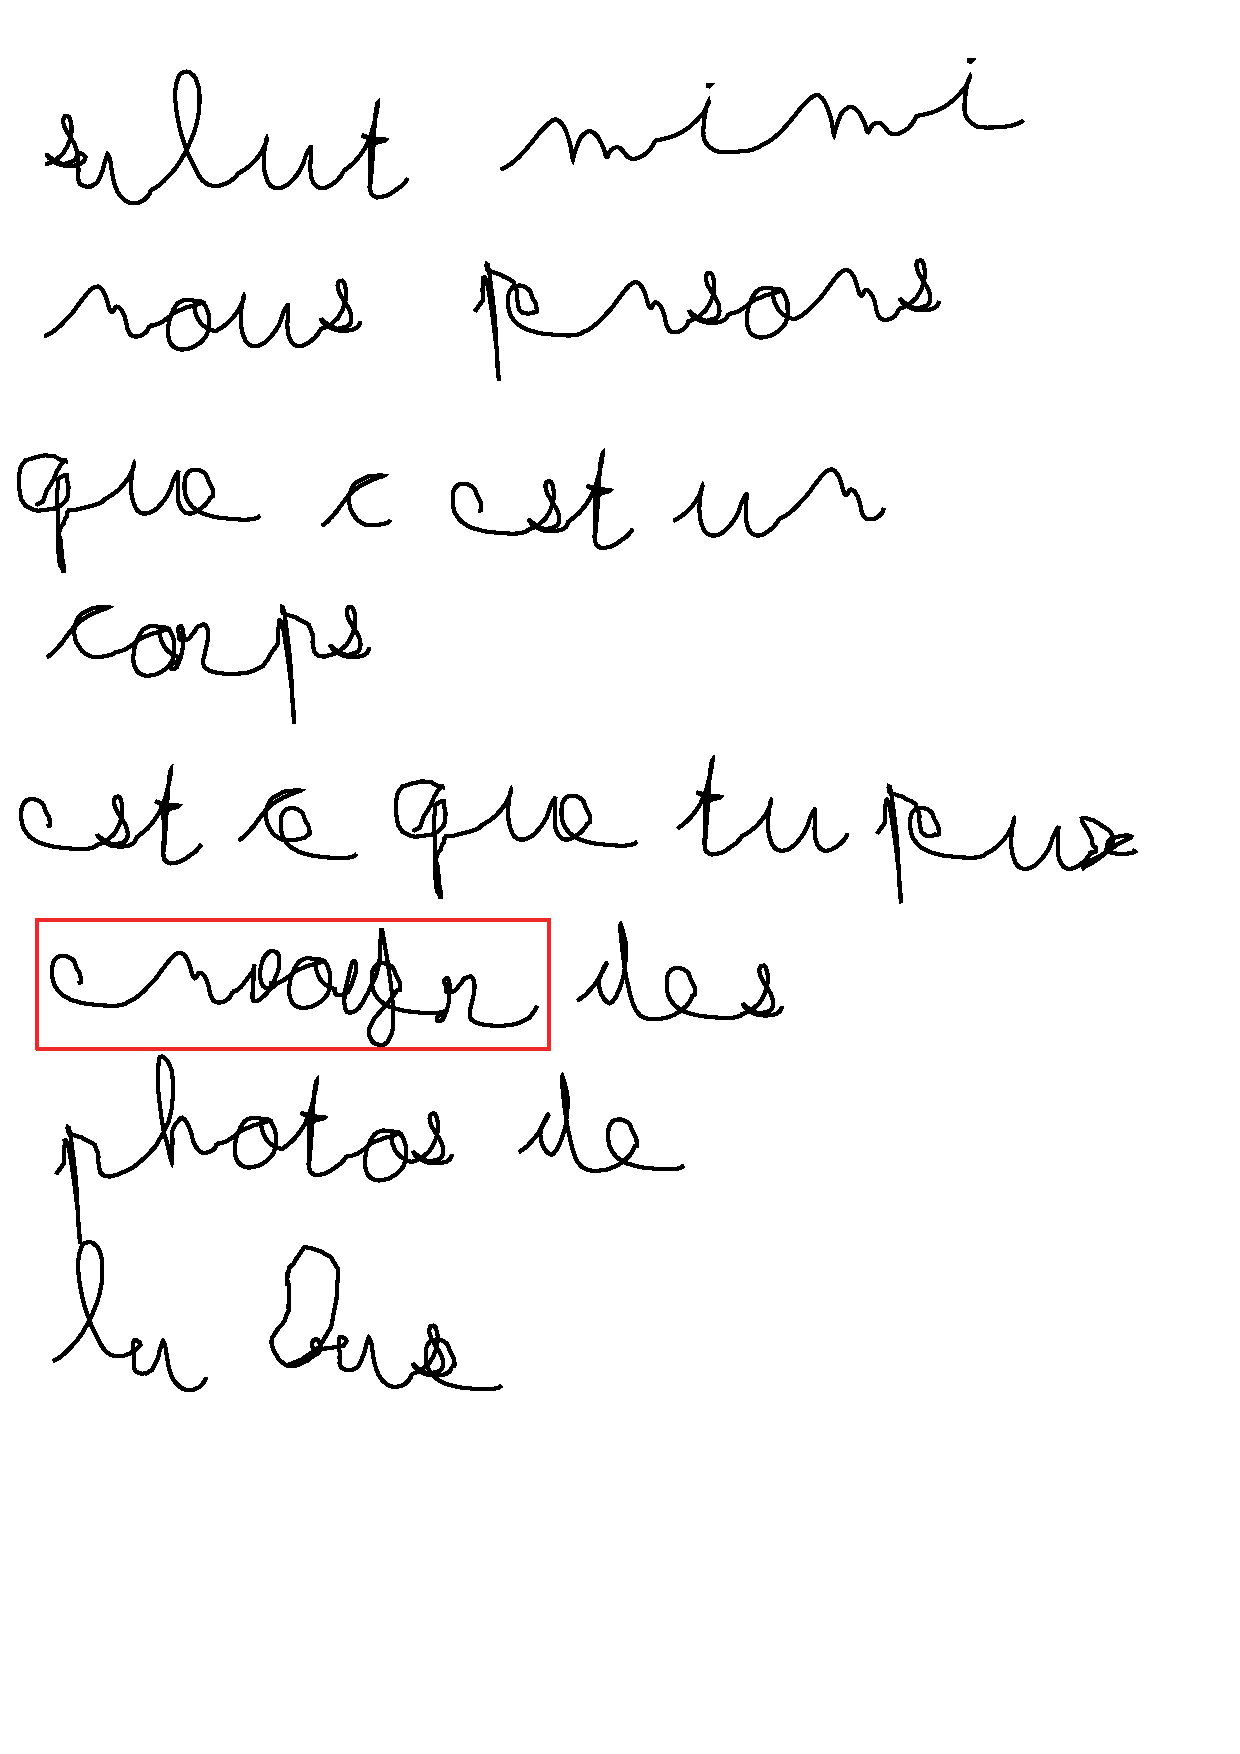
\includegraphics[width=0.43\linewidth]{cowriter/lettre-base-highlight}
            \hspace{1cm}%
        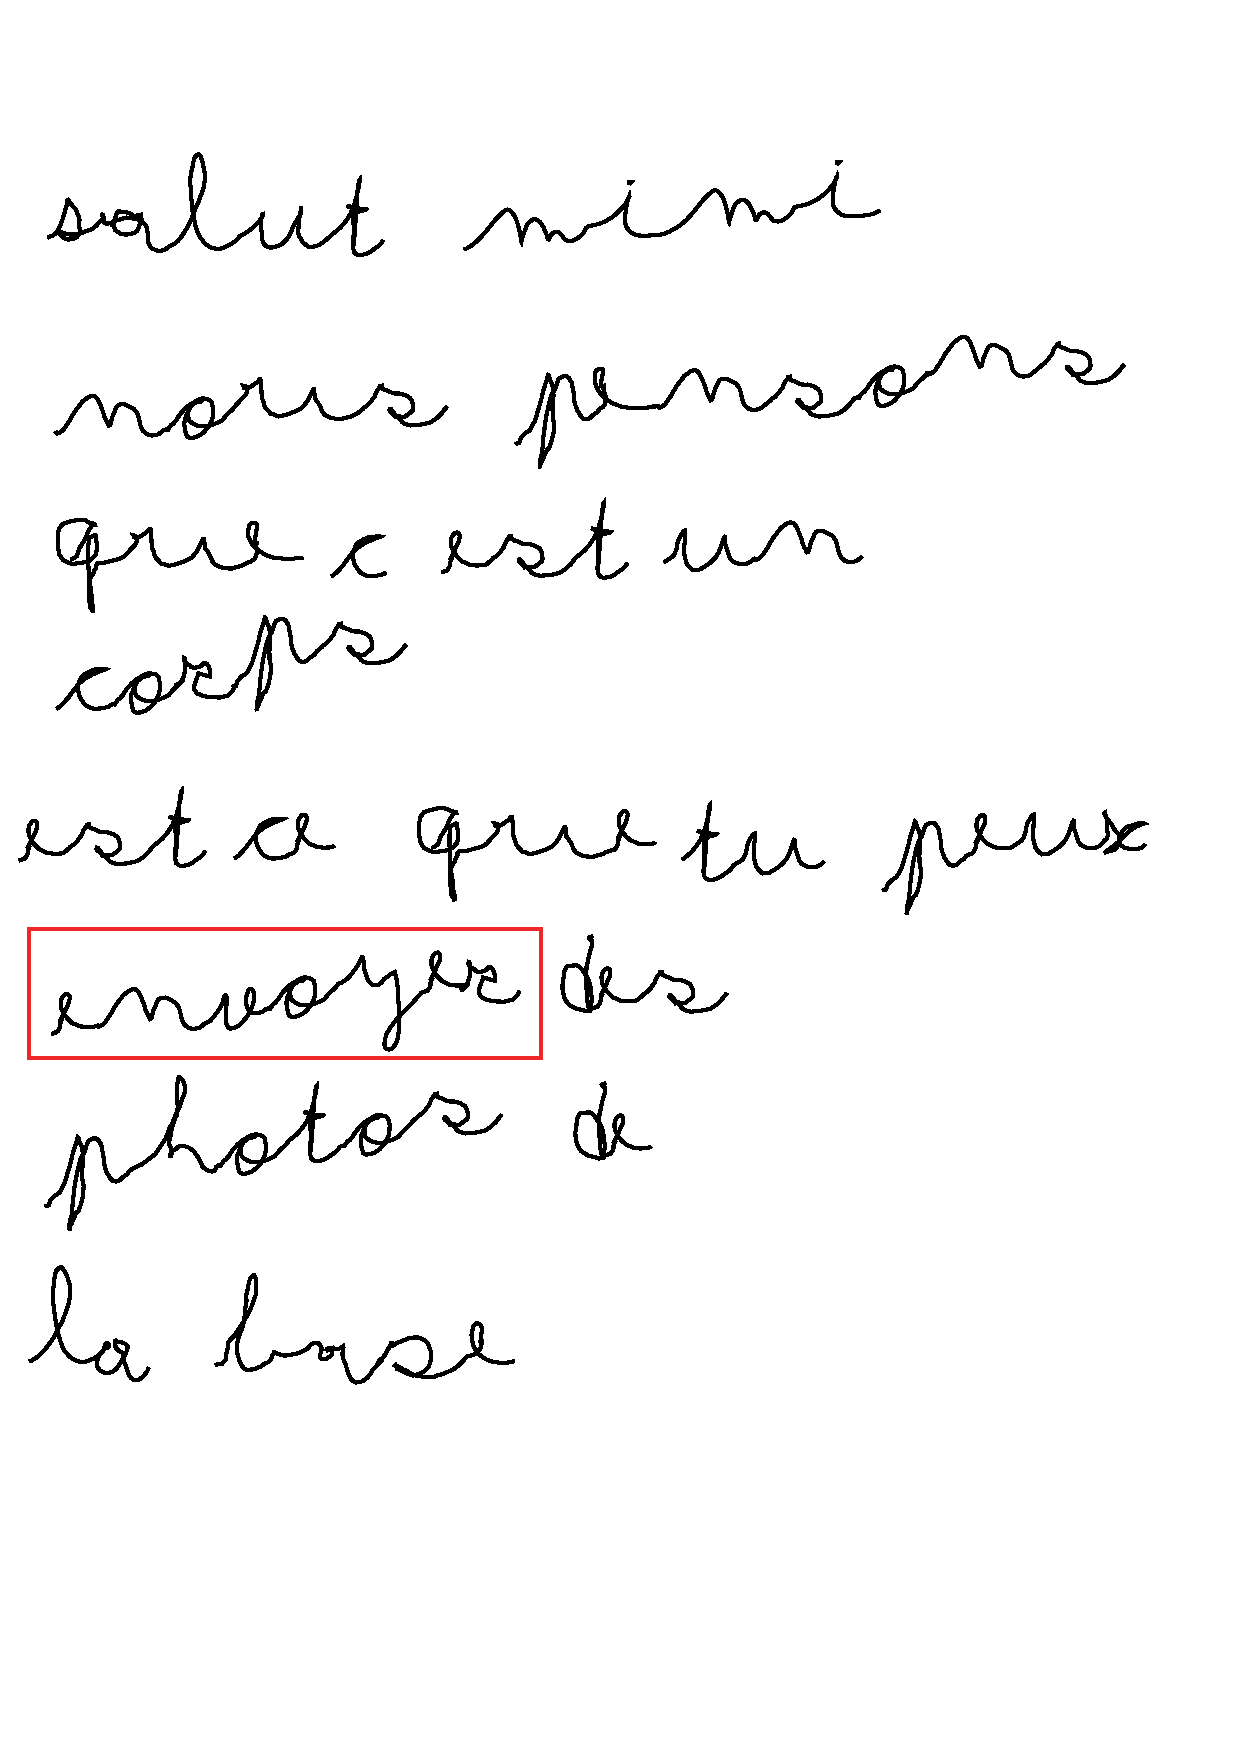
\includegraphics[width=0.43\linewidth]{cowriter/lettre-final-highlight}
        }
    \end{center}
    \badge{deana-epfl}
\end{frame}


\begin{frame}{What role does the robot play here?}
    \begin{itemize}
        \item<+-> The robot as 'cognitive agent' is key here (Protégé effect,
            metacognition)
        \item<+-> (note: a tool for the teacher vs a social agent for the child!)
        \item<+-> Could we replace it by someone else? Not easily. Have we
            just invented an original role for the robot?
    \end{itemize}
\end{frame}

\begin{frame}{A new space in the middle of the social spectrum?}

    \only<1-2>{
     \begin{center}
         \resizebox{\linewidth}{!}{
             \begin{tikzpicture}[stop jumping, >=latex]
                 \node[double arrow,draw] (spec) {Interaction spectrum};
                 \node<1->[minimum size=3cm,left=of spec] {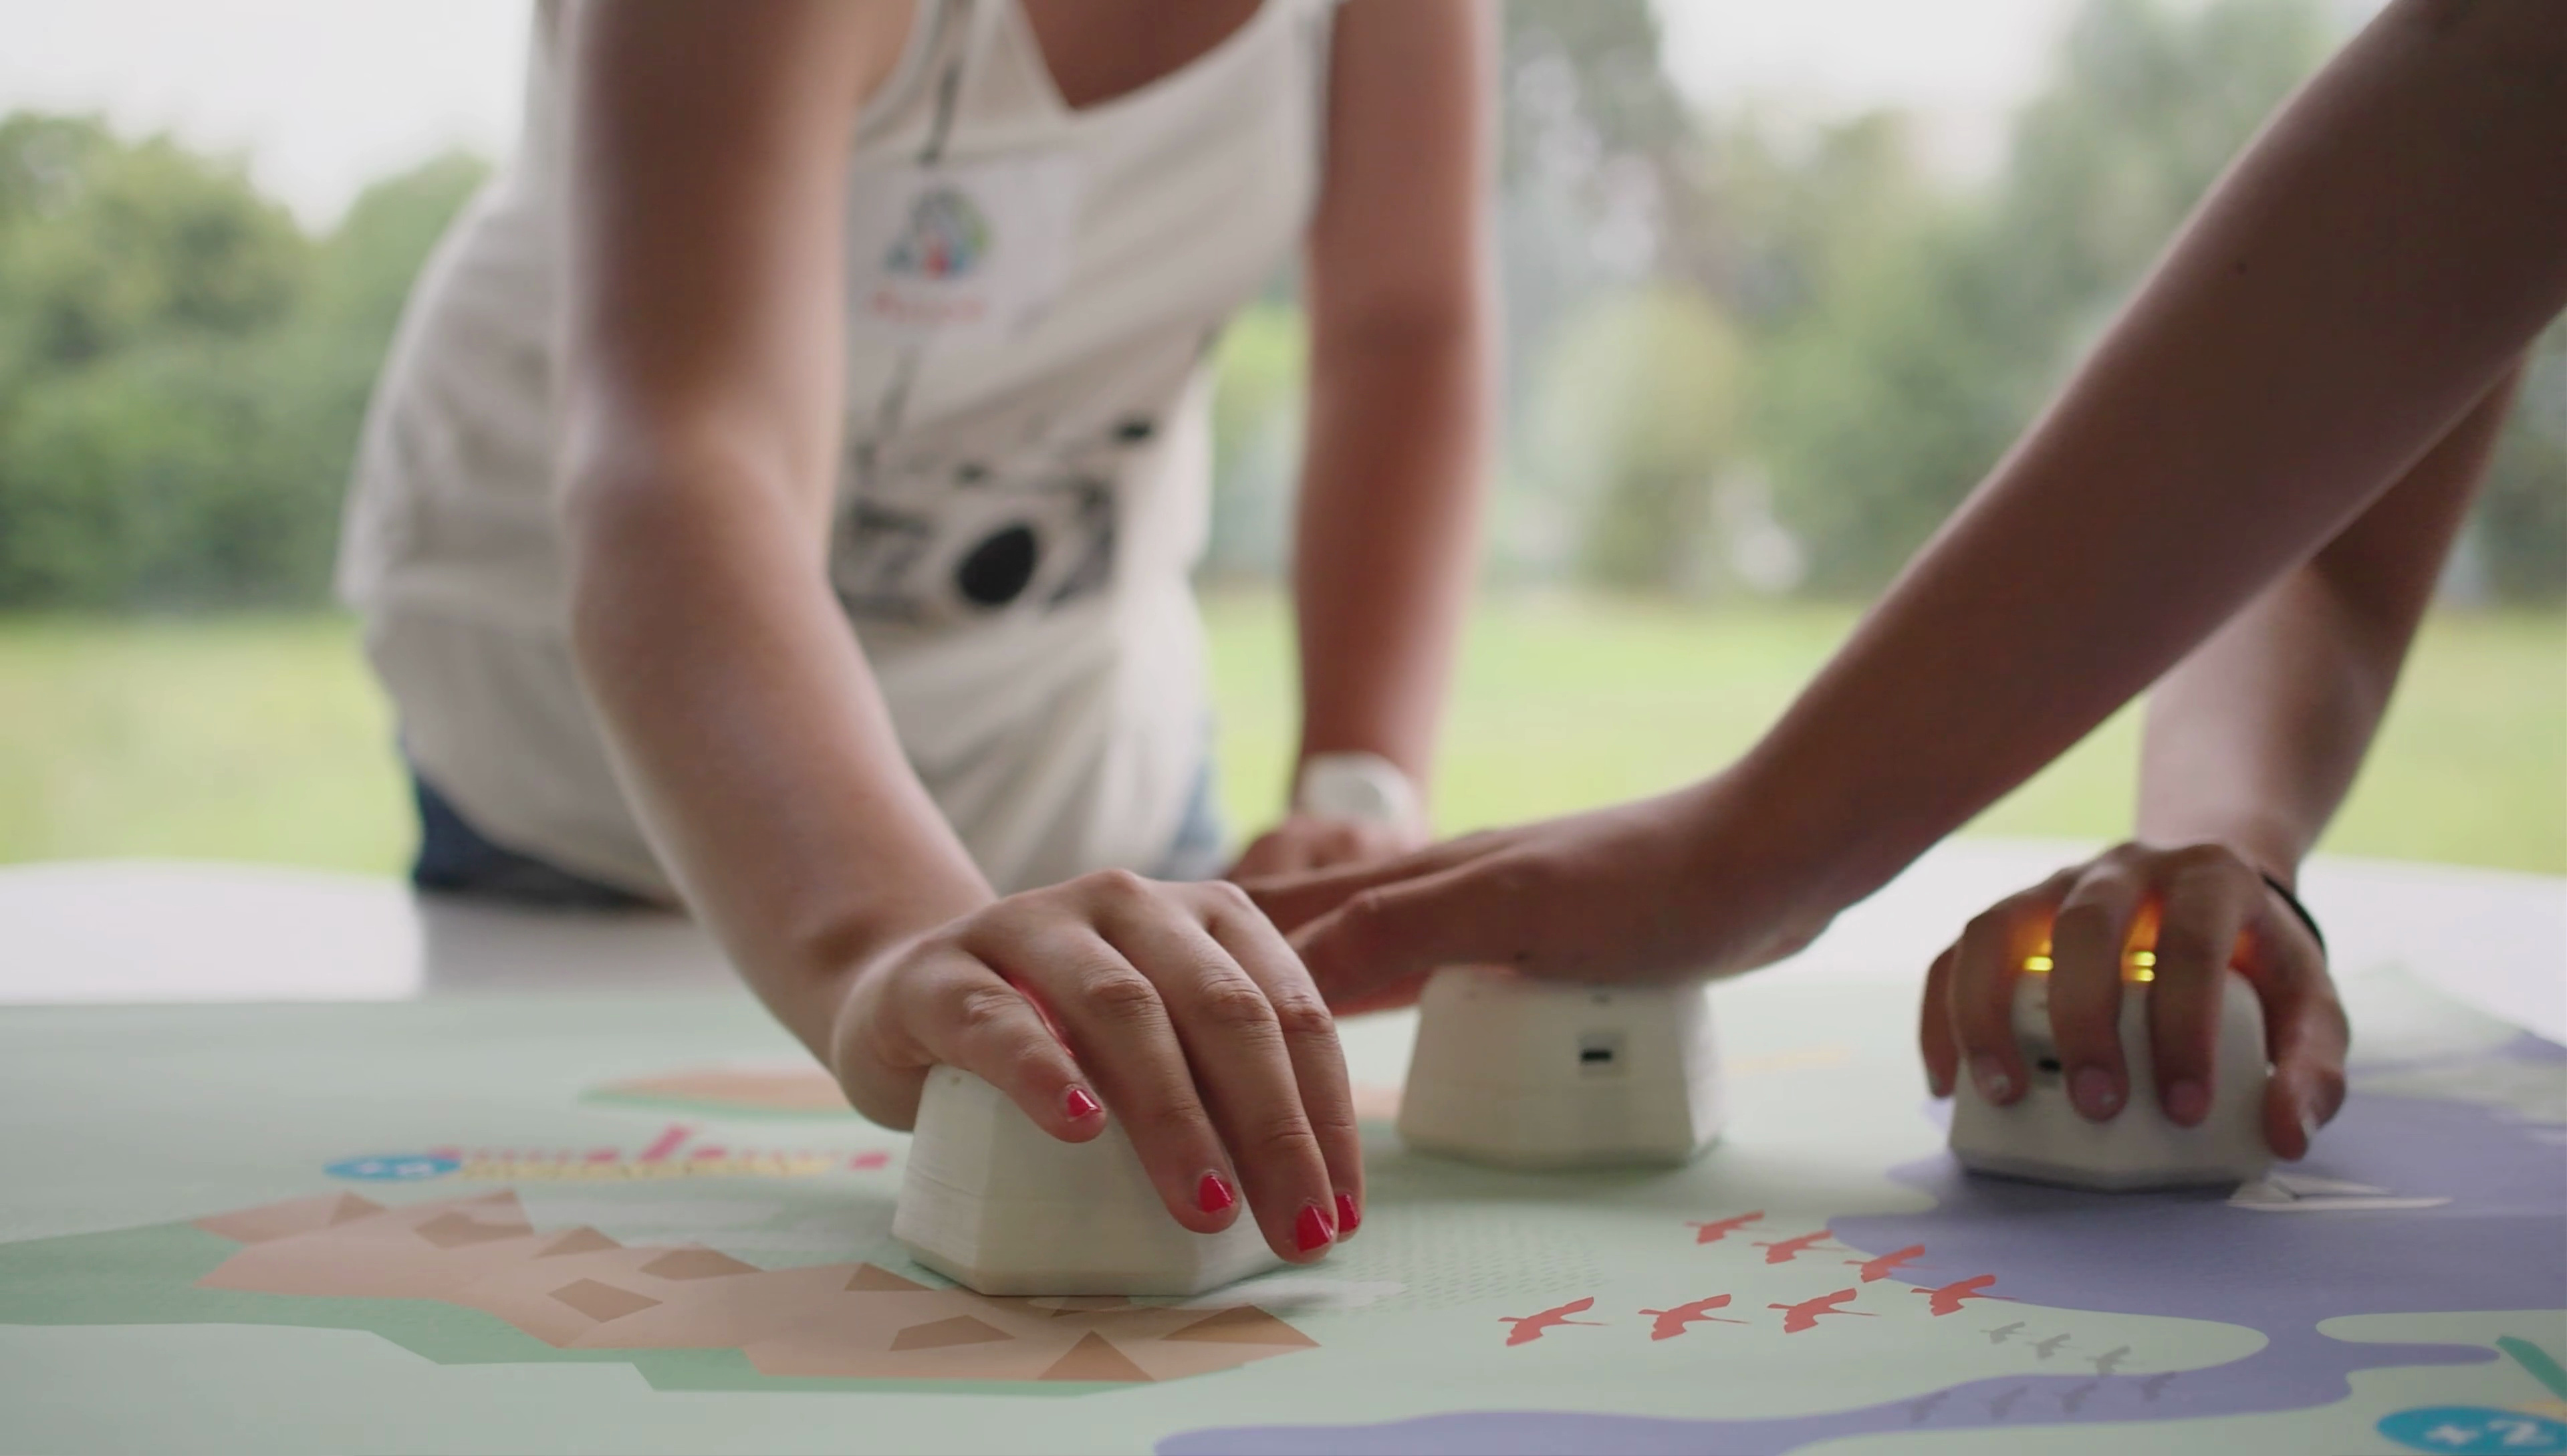
\includegraphics[width=5cm]{cellulo/haptic.jpg}};
                 \node<1->[minimum size=3cm,right=of spec] {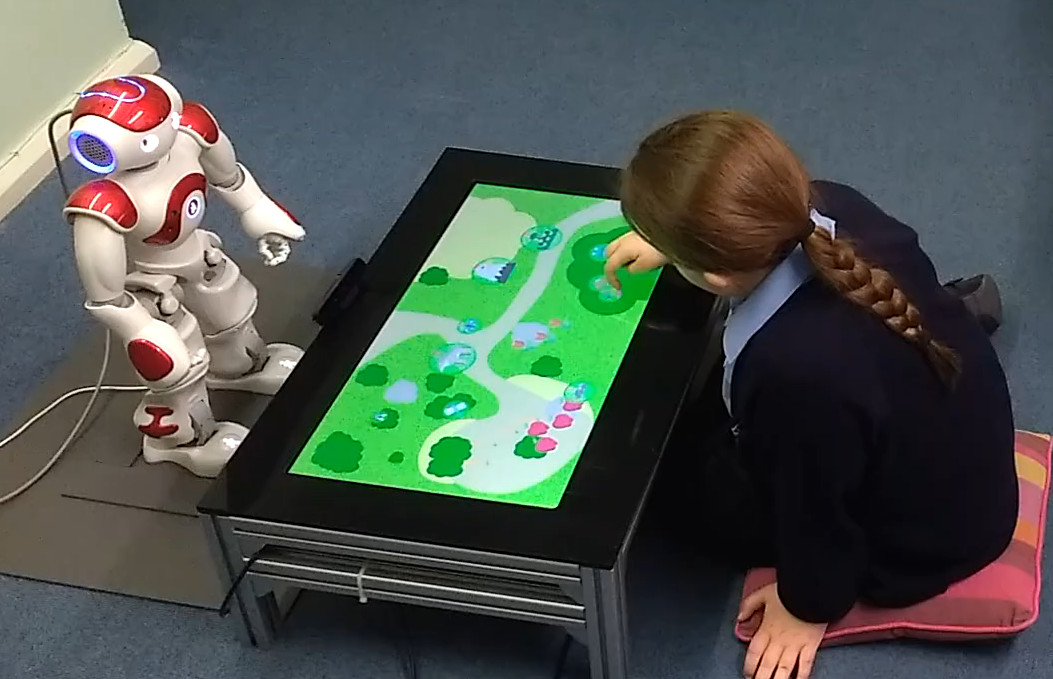
\includegraphics[width=5cm]{sparc/foodchain-game.jpg}};
                 \node<2>[minimum size=1cm,above=of spec]{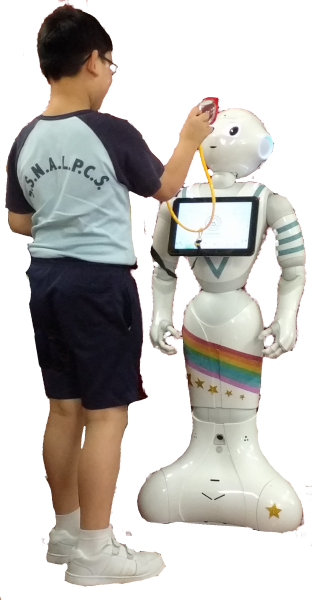
\includegraphics[height=5cm]{robot4SEN/child-pepper.png}};
             \end{tikzpicture}
         }
     \end{center}
    }

    \only<3>{

     Can we take the best of both world?

     \begin{itemize}
         \item purely a tool from the perspective of the teacher
         \item a (somewhat?) social agent from the perspective of the child
             $\rightarrow$ engagement, learning of social behaviours, etc
     \end{itemize}
   }
\end{frame}


%\begin{frame}[plain]
%
%    \begin{center}
%
%    {\Large\bf
%    But this is turn by turn!
%
%    What about less structured, ``messy'' interactions?
%    }
%
%    \pause
%
%    ...we are not yet very good at modelling real-world social dynamics...
%
%        \emph{Joint action} offers nevertheless a possible framework to reason
%        about it.
%    \end{center}
%\end{frame}
%
%\imageframe[scale=0.9]{joint-action-scenario}
%
%{
%    \paper{Lemaignan et al. {\bf Artificial Cognition for Social Human-Robot
%    Interaction: An Implementation} Artificial Intelligence 2017}
%\begin{frame}{Model-based joint action}
%    \badge{laas}
%    \begin{enumerate}
%        \item establish a joint goal
%        \item plan for the robot
%        \item plan for the human in order to build a set of priors
%        \item execute the robot plan
%        \item monitor progress of the partner towards the goal
%    \end{enumerate}
%
%    \pause
%
%    $\Rightarrow$ {\bf explicit cognitive steps}
%    \pause
%
%    \emph{...hard ones, though:
%    \begin{itemize}
%        \item how to communicate/agree on goals \& plans?
%        \item what about the human's own plans?
%        \item monitoring/recognising error situations
%        \item what to do when we're going 'off track'?
%        \item ...
%    \end{itemize}
%    }
%
%\end{frame}
%}
%
%
%{
%    \paper{Lemaignan et al. {\bf Artificial Cognition for Social Human-Robot
%    Interaction: An Implementation} -- Artificial Intelligence 2017}
%
%\begin{frame}{We can do a bit already}
%
%    \begin{center}
%    \only<1>{
%            \video{0.9\columnwidth}{figs/perspective-taking/this_box.webm?start=1}
%        }
%        \only<2>{
%            \video{0.9\columnwidth}{figs/underworlds/underworlds.mp4?start=20}
%        }
%    \end{center}
%
%    \badge{laas}
%\end{frame}
%
%}
%
%\begin{frame}{How do humans perform tasks together?}
%
%
%    \begin{center}
%        {\bf Collaborating is a costly socio-cognitive activity}.
%
%    \pause
%    Humans are good at it.
%        
%    They are also really good at minimizing the cost
%    involved.
%    \pause
%    
%        The key mechanism: {\bf prefer implicit to explicit}
%
%    \pause
%
%        ...which is closely related to: {\bf be lazy}
%        
%        First, go for the simple -- if possibly ambiguous -- actions; and, if
%        really needed, repair
%
%    \pause
%    \vspace{2cm}
%    {\bf What does ``be lazy'' mean for robots?}
%    \end{center}
%        
%\end{frame}
%
%\begin{frame}{One example: grounding of spatial language}
%
%
%    \begin{center}
%        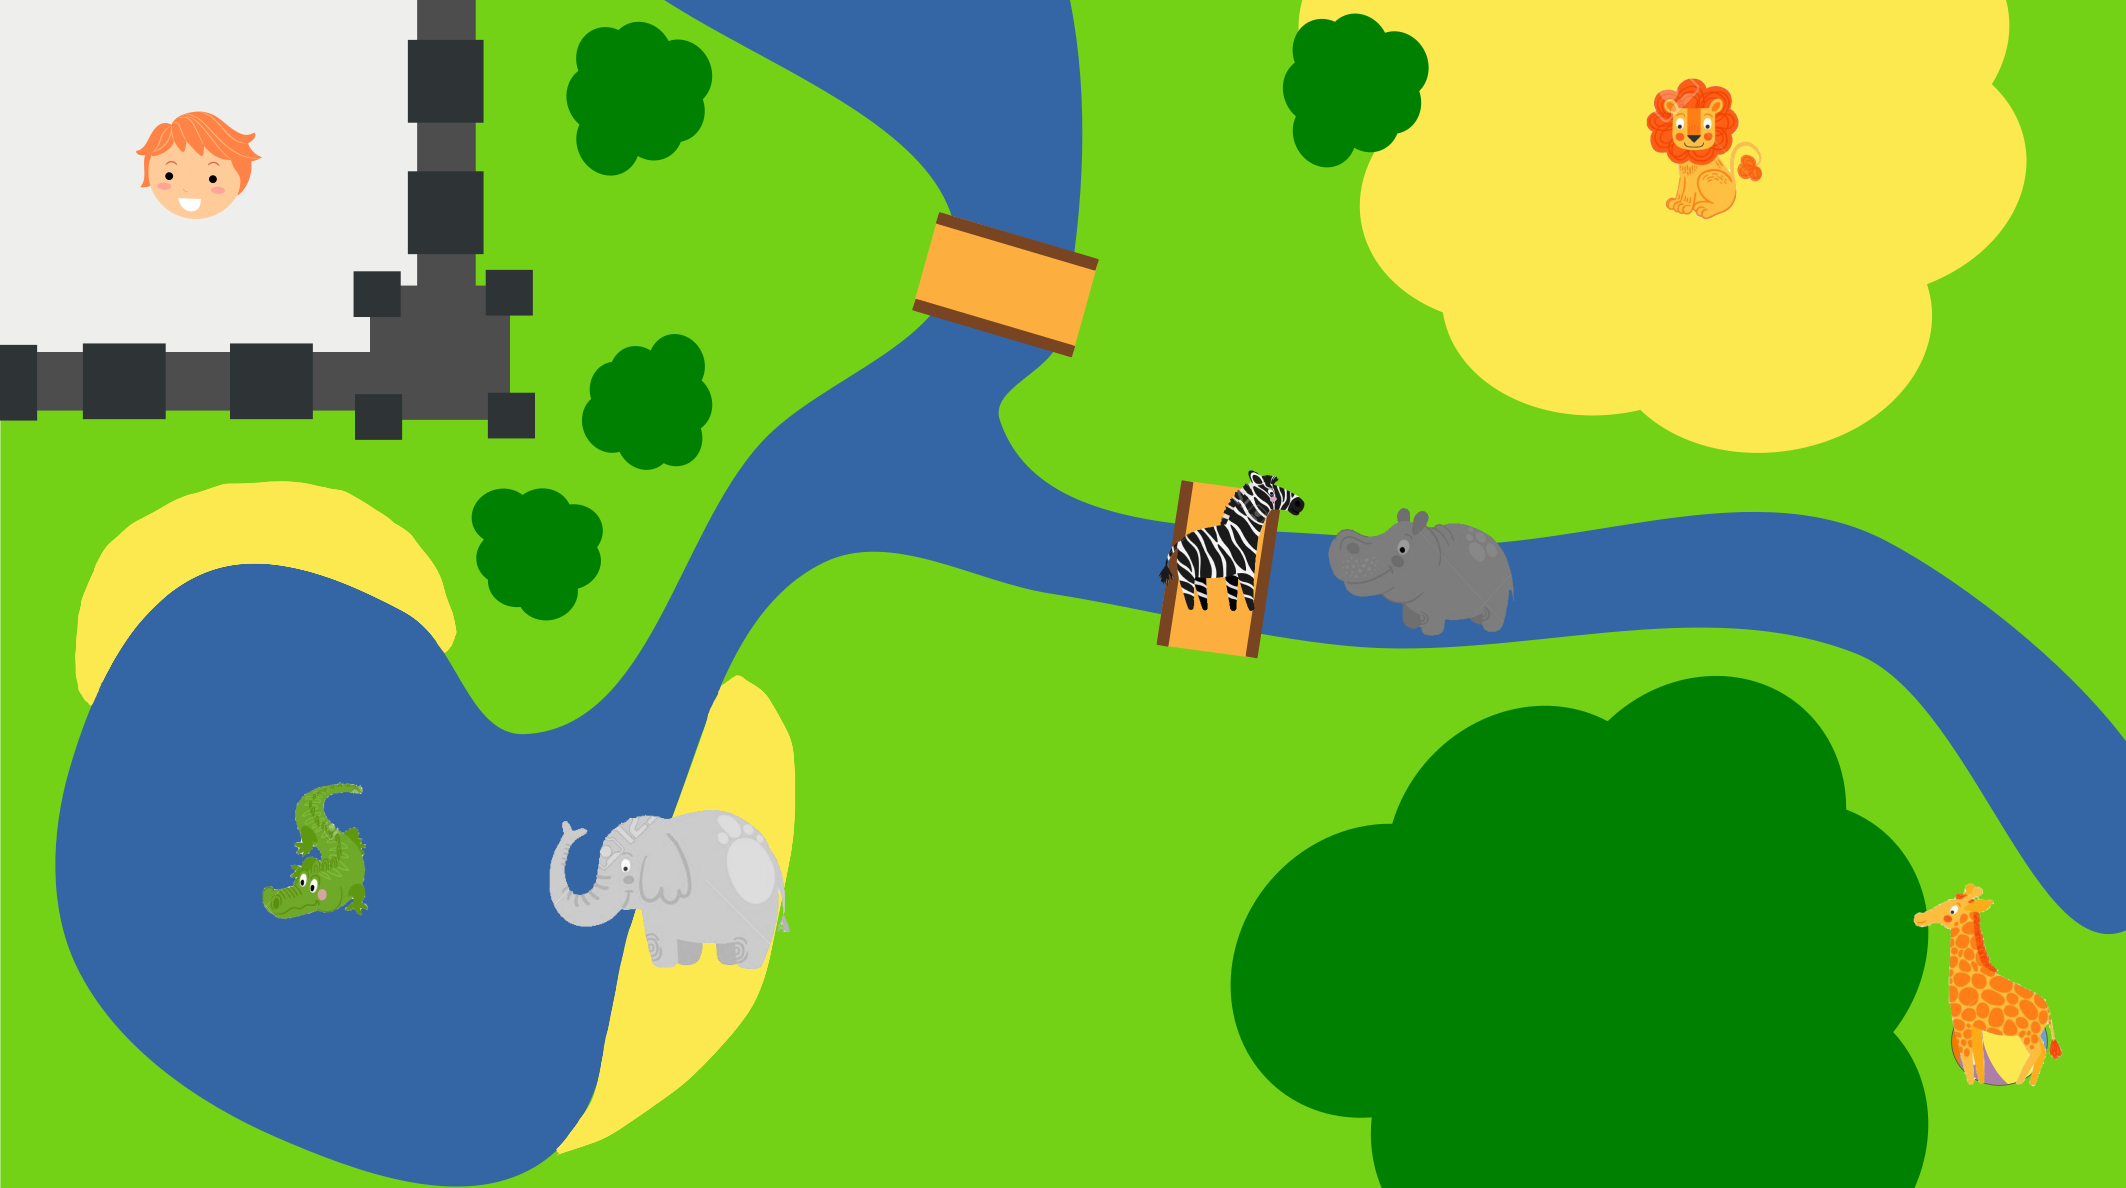
\includegraphics[width=0.9\linewidth]{ambiguous-desc/RefMap}
%
%    Ambiguities arise easily when describing spatial scenes.
%
%    How do we solve them?
%
%    \end{center}
%
%    \badge{chris}
%\end{frame}
%
%\imageframe[color=black]{ambiguous-desc/NosePointCropped}
%
%\imageframe{ambiguous-desc/LanguageUse}
%
%
%%\begin{frame}{}
%%    \begin{itemize}
%%        \item \emph{Ambiguous-Descriptive}: These statements provide details on
%%        the position of the object, but refer to more than one location,
%%        e.g. "The zebra is on a bridge."
%%        \item \emph{Contextual}: These are statements that follow on from a pre-
%%        vious statement or action, and would make no sense to a 3rd
%%        party who entered the conversation at the time the statement
%%        was made, e.g. "The other one."
%%        \item \emph{Negation}: This is when no statement is made other than to
%%        indicate the location chosen was incorrect, e.g."No".
%%        \item \emph{Non-Ambiguous}: These statements can only refer to one pos-
%%        sible location, e.g. "The lion is in the big sand pit."
%%    \end{itemize}
%%\end{frame}
%
%{\paper{Clark and Wilkes-Gibbs, \emph{Referring as a collaborative
%process}, Cognition 1986 \newline Pickering and Garrod, \emph{Alignment as the basis for successful
%communication}, Research on Language and Computation 2006}
%\begin{frame}{surface alignment; grounding criterion}
%
%    Psycholinguistics provides a lot of the foundational work on these
%    questions.
%
%    \begin{itemize}
%        \item<+-> \emph{Communication is a dynamic social process}: the partner often to signal
%            missing/misunderstood informations
%        \item<+-> Repairing is generally less costly than avoiding ambiguities in
%            the first place
%        \item<+-> You only ever need to reach the \emph{grounding criterion}, ie
%            \emph{enough} mutual understanding for the task
%        \item<+-> $\Rightarrow$ we typically only reach \emph{partial (or surface)
%            alignment} -- full alignment is usually not required
%        %\item<+-> {\bf do we need a high-level Theory of Mind at all?}
%    \end{itemize}
%\end{frame}
%}


\section{Assessing the interaction}


{
    \paper{Lemaignan et al. {\bf From Real-time Attention Assessment to “With-me-ness” in Human-Robot Interaction} HRI 2016}
\begin{frame}[label=withmeness]{Is the child engaging with the activity?}

    \Large
    \textbf{``With-me-ness''}: real-time estimation of surface engagement
\end{frame}
}

%%%%%%%%%%%%%%%%%%%%%%%%%%%%%%%%%%%%%%%%%%%%%%%%%%%%%%%%

\imageframe[color=black]{withmeness/realSetup}

%%%%%%%%%%%%%%%%%%%%%%%%%%%%%%%%%%%%%%%%%%%%%%%%%%%%%%%%

\imageframe[color=black]{withmeness/no-attention}

%%%%%%%%%%%%%%%%%%%%%%%%%%%%%%%%%%%%%%%%%%%%%%%%%%%%%%%%

\begin{frame}{Expected focus}

    \centering

    Example for the CoWriter task:

        \begin{multicols}{2}
           \scriptsize 
           \begin{tabular}{p{2.5cm}p{2.5cm}}
            \toprule
            {\bf Interaction Phase} & {\bf Expected targets} \\
            \midrule
            Presentation & {\sf robot} \\ 
            \midrule
            Waiting for word & {\sf secondary tablet} \\ 
            \midrule
            Writing word & {\sf tablet}\newline {\sf robot} \\ 
            \midrule
            Waiting for feedback & {\sf tablet}\newline {\sf secondary tablet} \\ 
            \midrule
            Story telling & {\sf robot} \\ 
            \midrule
            Bye & {\sf robot} \\ 
            \bottomrule
        \end{tabular}

            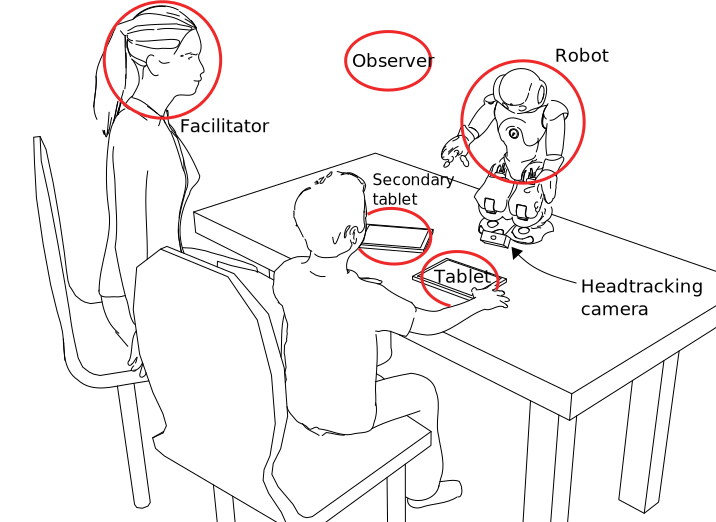
\includegraphics[width=0.95\columnwidth]{withmeness/experimental_setup}
        \end{multicols}

\end{frame}

%%%%%%%%%%%%%%%%%%%%%%%%%%%%%%%%%%%%%%%%%%%%%%%%%%%%%%%%

\imageframe[color=black]{withmeness/head_pose_real_world}

%%%%%%%%%%%%%%%%%%%%%%%%%%%%%%%%%%%%%%%%%%%%%%%%%%%%%%%%

{
\paper{Lemaignan et al. {\bf From Real-time Attention Assessment to “With-me-ness” in Human-Robot Interaction} HRI 2016}
\fullbackground[scale=0.95]{withmeness/with-me-ness-robot}

\begin{frame}{With-me-ness}
\end{frame}
}

%%%%%%%%%%%%%%%%%%%%%%%%%%%%%%%%%%%%%%%%%%%%%%%%%%%%%%%%

%{
%\paper{Lemaignan et al. {\bf From Real-time Attention Assessment to “With-me-ness” in Human-Robot Interaction} HRI 2016}
%\begin{frame}{With-me-ness is...}
%
%    {\bf With-me-ness is...}
%
%    \begin{itemize}
%        \item An {\bf objective} \& {\bf quantitative} precursor of engagement...
%        \item ...based on matching the {\bf user's focus of attention} with a set of
%            {\bf prior expectations}
%        \item Can be computed {\bf on-line} by the robot...
%        \item ...and {\bf sensitive to} the (task-dependent) {\bf set of
%            expectations}
%        \item $\Rightarrow$ {\bf relative} metric!
%    \end{itemize}
%
%
%\end{frame}
%}


 \begin{frame}[plain]{}

     {
     \centering
     \Large\bf

     Can we make one step further to understand what's going on when we
     interact?
     }

     \pause


    Most of our social and behavioural alignment comes from sub-conscious social
    mechanisms:

    \begin{itemize}
        \item entrainment (coupling), 
        \item mimicry, 
        \item implicit turn-taking,
        \item joint attention
        \item ...and others
    \end{itemize}
    \pause
    \begin{center}
        Let's observe them!
    \end{center}
\end{frame}


%\begin{frame}{The problem}
%    \begin{itemize}
%        \item These mechanisms are unfortunately often ill-defined, and
%            particularly difficult to turn into equations (or controllers, in
%            our case)
%        \item no close-form equation of social interactions $\Rightarrow$ data-driven approaches?
%    \end{itemize}
%\end{frame}
%
%\section[Data-driven!]{Towards the data-driven study of social dynamics}

%\begin{frame}{Data!}
%
%    If we want to use machine learning, we need data (relevant to child-robot
%    interactions in a learning environment).
%    
%    \pause
%
%    ...a task that exhibits:
%
%    \begin{itemize}
%        \item complex social dynamics
%        \item open, underspecified situations
%        \item natural interactions
%        \item rich semantics
%        \item interplay of many socio-cognitive functions
%    \end{itemize}
%
%    \pause
%
%    while being...
%    \begin{itemize}
%        \item reproducible/replicable experimental procedure
%        \item clear quantitative metrics
%        \item practical
%    \end{itemize}
%\end{frame}



\begin{frame}{Free play}

    \begin{center}
    {\Large ``Just play! Enjoy yourselves!''}
    \end{center}

    \vspace{3em}

    \begin{itemize}
        \item \textbf{rich set of cognitive and
            social dynamics}; importance of motivation/drive; \textbf{uncertain
            and unexpected situations}
        \item what is the right action policy? Focus instead on the \textbf{social policy}
    \end{itemize}
    \pause
    \begin{itemize}
        \item focus on children
        \item with a little bit of scaffolding \& framing
    \end{itemize}


\end{frame}
%
%\videoframe[0.56]{figs/freeplay/maud-zoe-pilot-edit.mkv?autostart&noaudio}
%
%{
%    \paper{Parten, {\bf Social participation among preschool children} Journal
%    of Abnormal and Social Psychology 1932}
%\begin{frame}[label=parten]{Stages of play}
%
%    In developmental psychology, Parten's {\bf stages of play}:
%
%    \begin{enumerate}
%        \item 
\includegraphics[height=1cm]{figs/stagesofplay/solitary} {\bf Solitary (independent) play}
%        \item 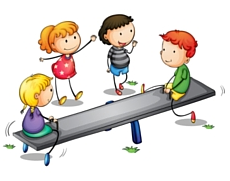
\includegraphics[height=1cm]{figs/stagesofplay/onlooker} {\bf Onlooker play}
%        \item 
\includegraphics[height=1cm]{figs/stagesofplay/parallel}{\bf Parallel play}
%        \item 
\includegraphics[height=1cm]{figs/stagesofplay/associative}{\bf Associative play}
%        \item 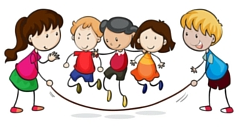
\includegraphics[height=1cm]{figs/stagesofplay/cooperative}{\bf Cooperative play}
%    \end{enumerate}
%
%    \note{
%    \begin{enumerate}
%        \item {\bf Solitary (independent) play}: Playing separately from
%            others, with no reference to what others are doing.
%        \item {\bf Onlooker play}: Watching others play. May engage in
%            conversation but not engaged in doing. True focus on the children at
%            play.
%        \item {\bf Parallel play} (adjacent play, social coaction): Playing
%            with similar objects, clearly beside others but not with them (near
%            but not with others.)
%        \item {\bf Associative play}:  Playing with others without
%            organization of play activity. Initiating or responding to
%            interaction with peers. 
%        \item {\bf Cooperative play}: Coordinating one’s behavior with that
%            of a peer. Everyone has a role, with the emergence of a sense of
%            belonging to a group. Beginning of "team work."
%    \end{enumerate}
%    }
%
%
%\end{frame}
%}
%
%\videoframe[0.56]{figs/freeplay/maud-zoe-pilot-edit.mkv?autostart&noaudio&start=28}
%
%\begin{frame}[plain]
%    \begin{center}
%    \Large\bf
%        Can we make it work for HRI?
%    \end{center}
%\end{frame}

%\imageframe[color=black, scale=0.9]{freeplay/sandbox}

\imageframe{freeplay/freeplay-overview2}

%\videoframe[0.56]{figs/kinematics_social_dynamics/clip_skel_01.mp4}
\videoframe[0.56]{figs/kinematics_social_dynamics/clip_01.mp4}

\videoframe[0.56]{figs/kinematics_social_dynamics/clip_skel_05.mp4}
\videoframe[0.56]{figs/kinematics_social_dynamics/clip_05.mp4}


%\imageframe[color=black]{freeplay/freeplay-sandbox-screenshot}
%\imageframe[color=black]{freeplay/analysis}

%
%\begin{frame}{'Sandboxed free play' experimental paradigm}
%
%    \begin{itemize}
%        \item \textbf{Structured methodology} (sandtray) yet \textbf{loosely structured
%            task} (free play)
%        \item<2-> physical playground $\rightarrow$ {\bf replaced by large
%            touchscreen}: escape perception and manipulation in
%            dense \& cluttered scene (but \emph{only} that)
%        \item<3-> importantly, \textbf{perception and interaction with the
%            partner is unimpaired}
%    \end{itemize}
%\end{frame}
%
%
%\imageframe[scale=0.9]{freeplay/setup_top}

%
%\begin{frame}{Social dynamics to be observed}
%
%    \begin{itemize}
%        \item<+-> the \textbf{task engagement}
%            \begin{itemize}
%                \item are the participants 'on task' or not?
%            \end{itemize}
%        \item<+-> the \textbf{interaction flow} \& \textbf{situation awareness}
%            \begin{itemize}
%                \item what is happening \emph{now}? what is the next expected
%                    action?
%            \end{itemize}
%        \item<+-> the \textbf{social attitude}
%            \begin{itemize}
%                \item pro-social, hostile, assertive (‘bossy’), passive...
%            \end{itemize}
%        \item<+-> the \textbf{social dynamics}
%            \begin{itemize}
%                \item entrainment (coupling), mimicry, implicit turn-taking, joint
%                    attention
%            \end{itemize}
%    \end{itemize}
%
%    \pause
%    $\rightarrow$ {\bf paradigm for socio-cognitive investigation}
%\end{frame}


%\section{Sandtray paradigm: more applications}
%
%\begin{frame}{Spatial reasoning and Perspective taking}
%    $\rightarrow$ on-going PhD work by Christopher Wallbridge
%    \begin{center}
%        \includegraphics<1>[width=0.9\linewidth]{spatial-relations/RefMap}
%        \includegraphics<2>[width=0.7\linewidth]{spatial-relations/placementcc}
%
%        \only<2>{(take home message: ambiguity is good for you!)}
%    \end{center}
%\end{frame}
%
%
%\begin{frame}{Supervised autonomy}
%    $\rightarrow$ on-going PhD work by Emmanuel Senft
%    \begin{center}
%        \includegraphics[width=0.9\linewidth]{sparc/sparc-setup}
%    \end{center}
%\end{frame}
%
%\section{The PInSoRo dataset}

%\imageframe{freeplay/freeplay-overview2}

%\begin{frame}{The PInSoRo dataset}
%    \begin{itemize}
%        \item 120 children, 4 to 8 years old
%        \item 75 interactions
%            \begin{itemize}
%                \item 90 children playing with another child, 
%                \item 30 playing with a robot
%            \end{itemize}
%        \item About 45h+ of recordings; 2M+ frames; $\approx$ 2TB
%         \item average duration of freeplay interactions: 24min in child-child
%         condition; 19min in child-robot condition
%    \end{itemize}
%
%    \begin{center}
%        Large open dataset: \href{https://freeplay-sandbox.github.io}{\bf freeplay-sandbox.github.io}
%    \end{center}
%\end{frame}

%
%\videoframe[0.56]{figs/mosaic_blend_long.mp4?autostart}
%
%\begin{frame}{Two baselines}
%
%    \begin{center}
%        \includegraphics<1>[width=\linewidth]{pinsoro-baselines}
%        \includegraphics<2>[width=\linewidth]{pinsoro-baselines2}
%    \end{center}
%\end{frame}

%\imageframe[color=black]{freeplay/3d-point-cloud-facial-features}


%\videoframe[0.56]{figs/bestof.mp4?autostart}

%\begin{frame}{Dataset}
%    \begin{itemize}
%        \item 120 children, 4 to 8 years old; 45h+ of recordings;
%     \item facial features extracted in ~98\% of frames
%    \end{itemize}
%
%    \begin{center}
%        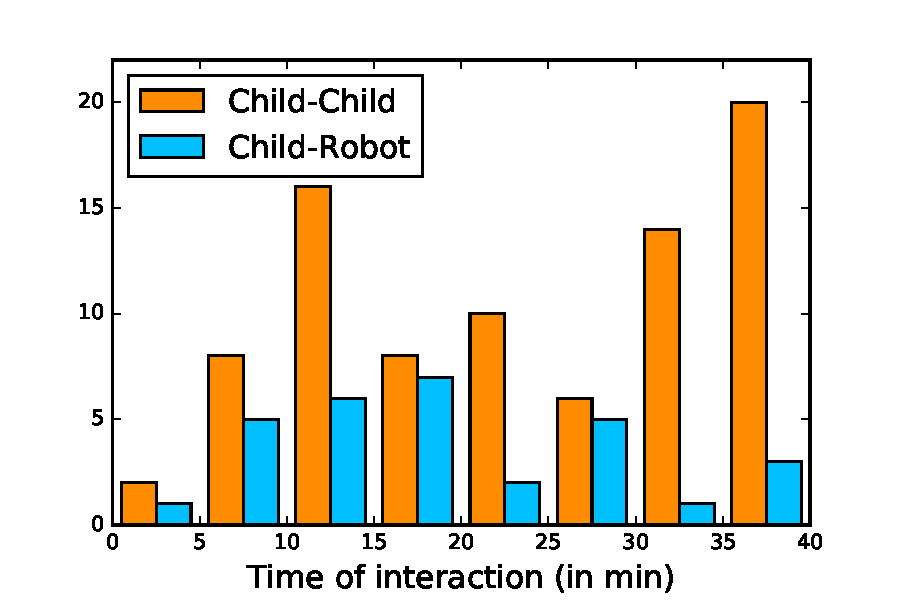
\includegraphics[width=0.5\linewidth]{freeplay/durations}
%    \end{center}
%\end{frame}

%\imageframe[color=black]{freeplay/rviz-faces}
%\videoframe[0.56]{figs/optical_flow.mp4?autostart}

{
    \paper{Lemaignan et al. {\bf The PInSoRo
    dataset: Supporting the data-driven study of child-child and child-robot
    social dynamics} PLOS One 2018}
\begin{frame}{13000+ annotations}
    \begin{center}
        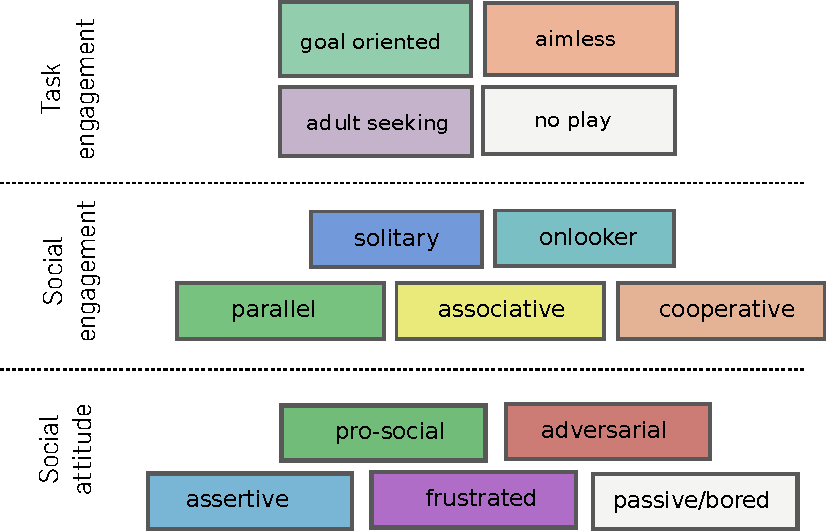
\includegraphics[width=0.8\linewidth]{freeplay/coding-scheme}
    \end{center}
\end{frame}
}
\note{
Coding scheme for social attitude derives from the Social Communication Coding System (SCCS) 
}

%\imageframe[scale=0.95, color=black]{freeplay/annotator}
%
%\begin{frame}{Social annotations}
%    So far,
%    \begin{itemize}
%        \item 85\% of the dataset annotated
%        \item 11500+ annotations
%        \item average duration of coded episodes: 46 seconds
%        \item 22\% double-coded
%    \end{itemize}
%\end{frame}
%

\videoframe[0.56]{figs/pinsoro/annotations.mp4?autostart}
\videoframe[0.56]{figs/pinsoro/pinsoro-matplotlib.mp4?autostart}

%\begin{frame}[plain]
%    \Large
%    \begin{center}
%        Anonymised version (5.7GB) available on-line. Grab it now!
%
%        \LARGE \href{https://freeplay-sandbox.github.io}{\bf freeplay-sandbox.github.io}
%
%        \vspace{3cm}
%            \large Open data! Hosted on EU's  
\includegraphics[width=0.3\linewidth]{zenodo}
%    \end{center}
%\end{frame}

\imageframe[caption={200 participants}]{kinematics_social_dynamics/questionnaire.png}
\imageframe{kinematics_social_dynamics/dataset.png}

\begin{frame}{Three constructs to rule them all}
        \centering
        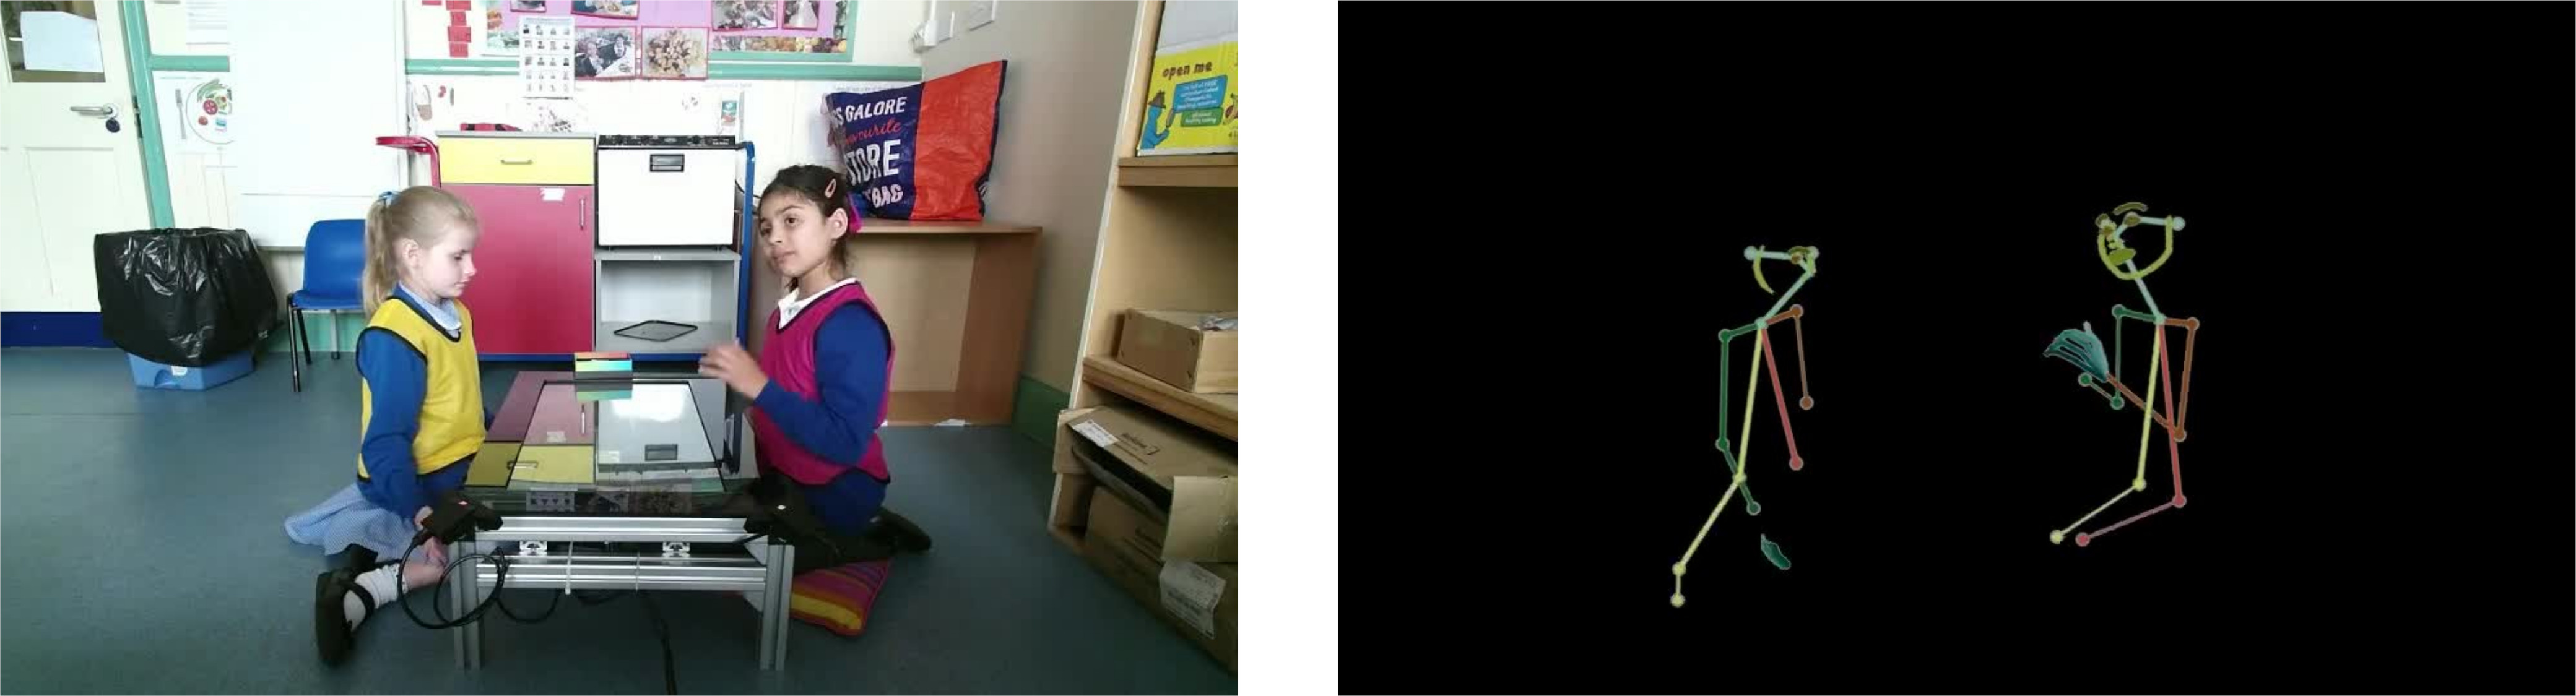
\includegraphics[width=0.9\linewidth]{kinematics_social_dynamics/clips.jpg}

    \textbf{Interaction imbalance}
    
    \textbf{Interaction valence}
    
    \textbf{Engagement}

\end{frame}



%%%%%%%%%%%%%%%%%%%%%%%%%%%%%%%%%%%%%%%%%%%%%%%%%%%%%%%%
%%%%%%%%%%%%%%%%%%%%%%%%%%%%%%%%%%%%%%%%%%%%%%%%%%%%%%%%
%%%%%%%%%%%%%%%%%%%%%%%%%%%%%%%%%%%%%%%%%%%%%%%%%%%%%%%%

%\section[For HRI?]{What does this dataset mean to HRI?}
%
%\imageframe[caption=Mutual gaze? Joint attention?]{freeplay/setup-child-child}
%
%\begin{frame}{Training for gaze estimation}
%
%    \Large End-to-end training to map 2D facial features to gaze location
%
%    \begin{center}
%        \includegraphics[width=0.9\linewidth]{nn-gaze-estimation}
%    \end{center}
%
%    \begin{itemize}
%        \item \textbf{Input}: 32 2D points (eyes, eyebrows, nose, ears,
%            shoulders)
%        \item \textbf{Output}: 2D gaze location on the interactive table
%    \end{itemize}
%\end{frame}
%
%\imageframe[color=black]{visual_tracking}
%
%\begin{frame}{Training for gaze estimation}
%
%    \Large End-to-end training to map 2D facial features to gaze location
%
%    \begin{center}
%        \includegraphics[width=0.9\linewidth]{nn-gaze-estimation}
%    \end{center}
%
%    \begin{itemize}
%        \item \textbf{Pros}: no calibration; no eye tracking device; 2D images
%        \item \textbf{Cons}: require a initial ground truth; accurate?
%    \end{itemize}
%\end{frame}
%
%\imageframe[color=black]{visual_tracking_size}
%\videoframe[0.56]{figs/gaze_tracking_distribution.mkv}
%\videoframe[0.40]{figs/gaze_tracking.ogv?autostart}
%
%
%\begin{frame}[plain]
%    \begin{center}
%    \Large\bf
%        What about social HRI?
%    \end{center}
%\end{frame}
%%%%%%%%%%%%%%%%%%%%%%%%%%%%%%%%%%%%%%%%%%%%%%%%%%%%%%%%%%%%%%%%%%%%
%%%%%%%%%%%%%%%%%%%%%%%%%%%%%%%%%%%%%%%%%%%%%%%%%%%%%%%%%%%%%%%%%%%%
%%%%%%%%%%%%%%%%%%%%%%%%%%%%%%%%%%%%%%%%%%%%%%%%%%%%%%%%%%%%%%%%%%%%
%\section[DNNs]{Deep learning and robotics}
%
%{
%    \paper{Mnih et al. {\bf Human-level control through deep reinforcement learning} -- Nature 2015}
%\begin{frame}{Learning Complex Behaviours}
%
%    \begin{center}
%        \includegraphics[width=\linewidth]{breakout}
%    \end{center}
%
%
%        \begin{itemize}
%            \item Inputs: raw screen image + score
%            \item from the outside, looks like planning
%            \item<2-> \sout{1.000.000} {\bf 500} games to play a good human-level
%        \end{itemize}
%
%\end{frame}
%}
%
%\videoframe[0.56]{figs/ogata-deeplearning-towel-folding.mp4?autostart&noaudio&start=19}
%
%{
%    \paper{Yang et al. {\bf Repeatable Folding Task by Humanoid Robot Worker using
%    Deep Learning} -- Robotics and Automation Letters 2017}
%\begin{frame}{Learning sequences}
%
%    Ogata's demonstration (published this year in IEEE RAL):
%
%    \begin{itemize}
%        \item 2 arms, 12 DoF
%        \item Inputs: on-board 112$\times$112px camera, joint state
%        \item<2-> training from 40 teleoperated demonstrations of $\approx$70s
%
%    \end{itemize}
%
%    \onslide<3>{
%
%    Not only learning poses, but \textbf{sequences as well}.
%    
%    \emph{Time-Delay Neural Network} (TDNN) to learn to
%    predict the next step (no RNNs!).
%}
%\end{frame}
%}

%%%%%%%%%%%%%%%%%%%%%%%%%%%%%%%%%%%%%%%%%%%%%%%%%%%%%%%%%%%%%%%%%%%%%%%%%%%%%%%
%%%%%%%%%%%%%%%%%%%%%%%%%%%%%%%%%%%%%%%%%%%%%%%%%%%%%%%%%%%%%%%%%%%%%%%%%%%%%%%
%%%%%%%%%%%%%%%%%%%%%%%%%%%%%%%%%%%%%%%%%%%%%%%%%%%%%%%%%%%%%%%%%%%%%%%%%%%%%%%
%%%%%%%%%%%%%%%%%%%%%%%%%%%%%%%%%%%%%%%%%%%%%%%%%%%%%%%%%%%%%%%%%%%%%%%%%%%%%%%

%\begin{frame}{What do you see?}
%    \badge{maddy}
%
%    20 30-secs clips with a range of social situations; 200 participants on
%    m-turk.
%
%    t-test between skeleton only and full video-streams show no difference in
%    perception for the vast majority of the 11 tested constructs (cooperative,
%    competitive, friendly, sad, engaged,...).
%
%    \only<1>{
%    \begin{center}
%        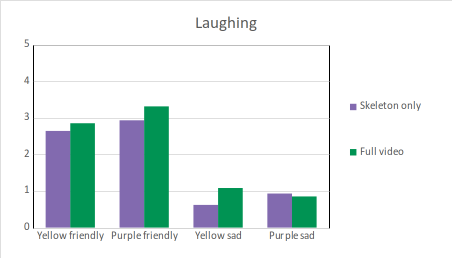
\includegraphics[width=0.4\linewidth]{kinematics_social_dynamics/constructs-laughing}
%        \hspace{1cm}
%        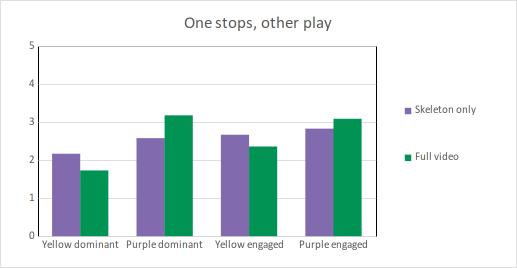
\includegraphics[width=0.45\linewidth]{kinematics_social_dynamics/constructs-one-stops-other-play}
%    \end{center}
%
%    }
%    \only<2>{
%
%    {\bf $\Rightarrow$ 30-secs long sequences of body postures and facial landmarks
%    of dyads should be sufficient to recognise a social situation}
%    }
%
%
%\end{frame}
%
%\begin{frame}{Data crunching going on!}
%    \begin{center}
%        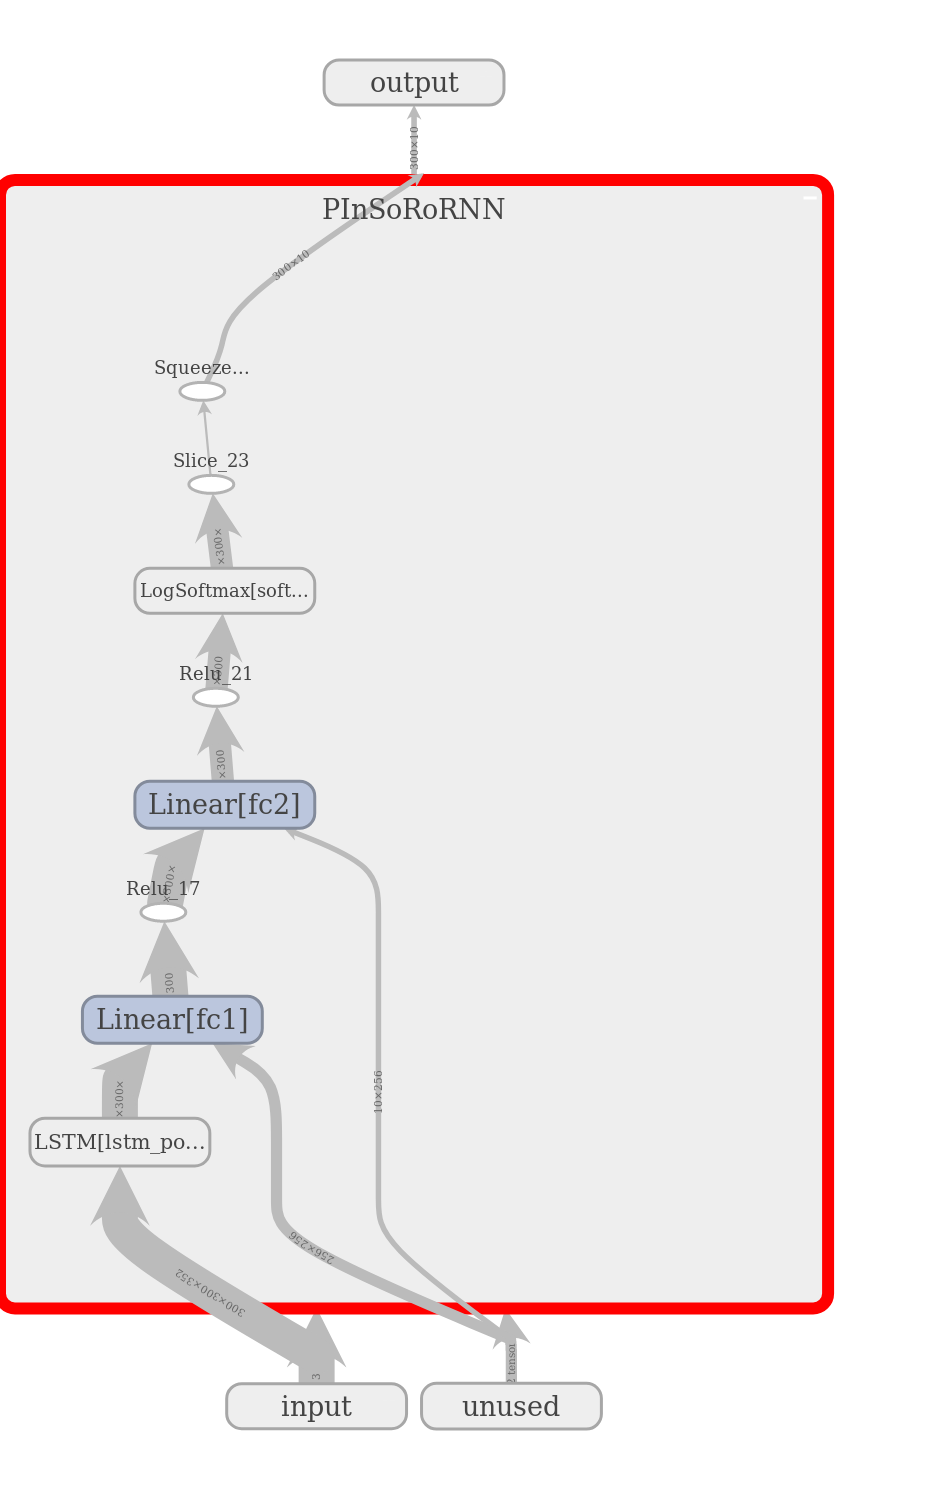
\includegraphics[width=0.35\linewidth]{pinsoronet/pinsoro-net-v2}
%        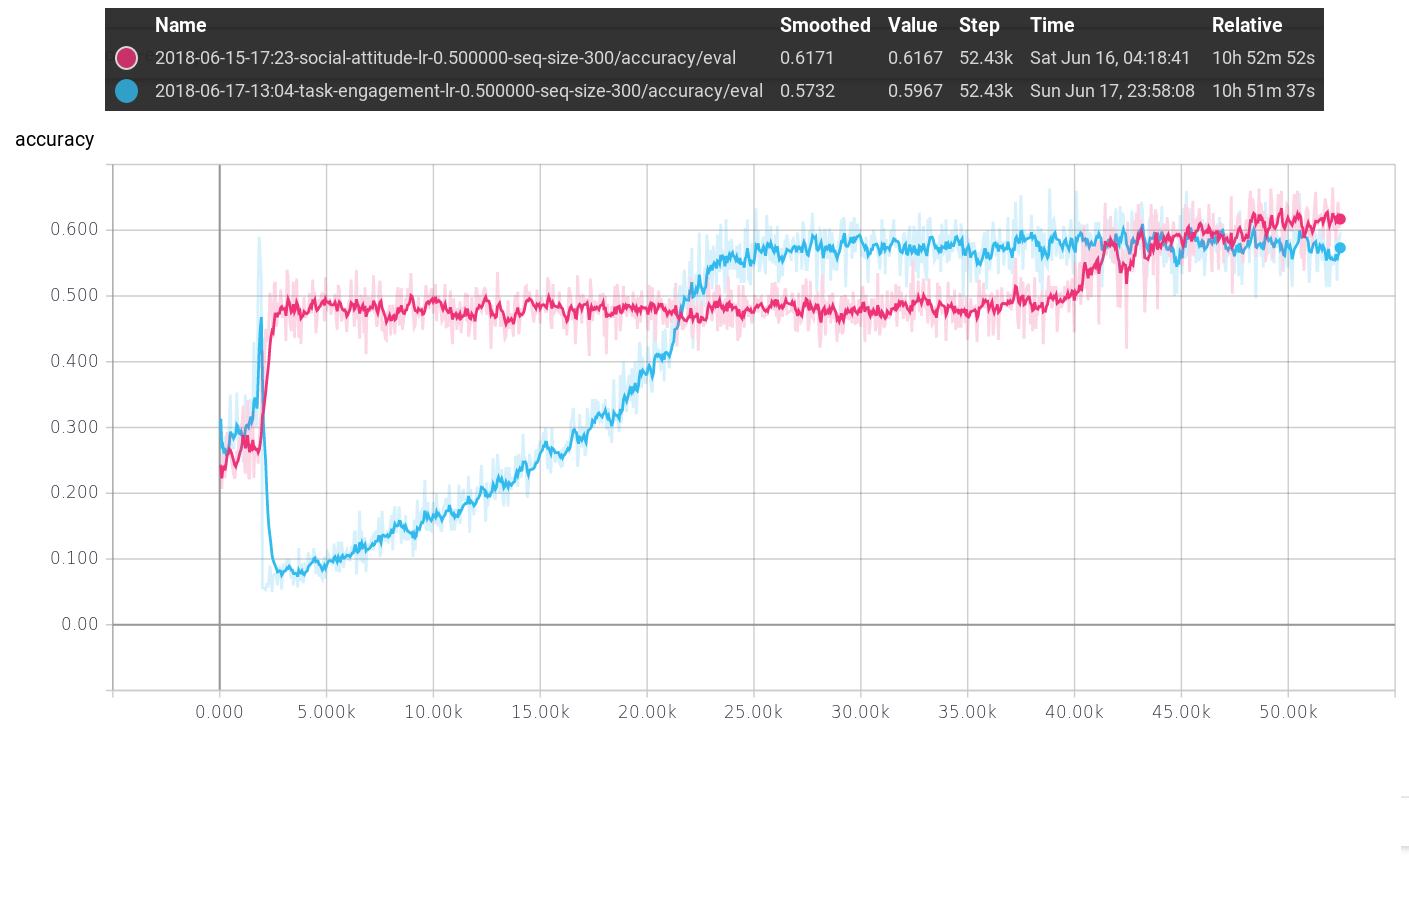
\includegraphics[width=0.6\linewidth]{pinsoronet/pinsoronet-v2-accuracy-social-attitude-task-engagement}
%    \end{center}
%
%    pytorch; trained on 10 epochs x 2M datapoints; {\bf WIP!!}
%\end{frame}


%\videoframe[0.56]{figs/annotations.mp4?autostart&start=10}


\begin{frame}{Our goal}

    {\bf Real-time identification} by the robot of...

    \begin{itemize}
        \item<+-> the \textbf{task engagement}
            \begin{itemize}
                \item is my partner 'on task' or not?
            \end{itemize}
        \item<+-> the \textbf{interaction flow} \& \textbf{situation awareness}
            \begin{itemize}
                \item what is happening right now? should I do something?
            \end{itemize}
        \item<+-> the \textbf{social attitude}
            \begin{itemize}
                \item Pro-social, hostile, assertive (‘bossy’), passive...
            \end{itemize}
        \item<+-> the \textbf{social dynamics}
            \begin{itemize}
                \item entrainment (coupling), mimicry, turn-taking, joint
                    attention
            \end{itemize}
    \end{itemize}

    \pause

    Social behaviours; Social dynamics: \textbf{generation as well!}
\end{frame}


%{
%    \fullbackground[color=black]{pinsoro/annotations-skel}
%\begin{frame}[plain]
%
%    \vspace{7cm}
%
%\setbeamercolor{hriSec1Demo}{fg=white!70!black}
%\begin{beamercolorbox}[wd=\linewidth,ht=6ex,dp=0.7ex]{hriSec1Demo}
%
%    The problem is framed, data is available, next step: {\bf mining it!}
%\end{beamercolorbox}
%\end{frame}
%}
%

%%%%%%%%%%%%%%%%%%%%%%%%%%%%%%%%%%%%%%%%%%%%%%%%%%%%%%%%%%%%%%%%%%%%%%%%%%%%%%%
%%%%%%%%%%%%%%%%%%%%%%%%%%%%%%%%%%%%%%%%%%%%%%%%%%%%%%%%%%%%%%%%%%%%%%%%%%%%%%%
%%%%%%%%%%%%%%%%%%%%%%%%%%%%%%%%%%%%%%%%%%%%%%%%%%%%%%%%%%%%%%%%%%%%%%%%%%%%%%%
%%%%%%%%%%%%%%%%%%%%%%%%%%%%%%%%%%%%%%%%%%%%%%%%%%%%%%%%%%%%%%%%%%%%%%%%%%%%%%%

%\section[Conclusion]{Back to the bigger picture}
%
%\begin{frame}{One question}
%
%    \Large
%    \centering
%
%    {\bf Can sociality emerge from interaction?}
%
%    \pause
%    \normalsize
%    \vspace{2em}
%
%    Both ``emerge'' as \emph{arise from} and ``emerge`` as in \emph{emergent paradigm of
%    cognition}
%
%    \pause
%
%    ``Social cognition arising in interaction''? $\rightarrow$ a situated \&
%    embodied view on cognition
%
%\end{frame}
%
%\begin{frame}{Deep learning of social interactions}
%
%    \large
%
%    \begin{center}
%
%    Working hypothesis: \textbf{Sociality emerges from interaction}
%
%
%    \pause
%
%    $\Rightarrow$ {\bf learning how to interact might lead to an emergent
%    socio-cognitive behaviour}
%   
%    \pause
%
%    $\Rightarrow$ {\bf (Deep) learning of socio-cognitive human-robot interactions}
%
%
%
%    \normalsize
%
%        (Supervised (or unsupervised!) recurrent neural networks to model others'
%            minds $\rightarrow$ a connectionist theory of mind!)
%
%
%    \pause
%    \vspace{2em}
%    {\bf ...towards a principled model of social cognition?}
%
%    \end{center}
%
%\end{frame}
%
%%%%%%%%%%%%%%%%%%%%%%%%%%%%%%%%%%%%%%%%%%%%%%%%%%%%%%%%%
%
%{
%    \paper{cited in Lewandowsky and Farrell, {\bf Computational Modeling In
%    Cognition}, 2011}
%\begin{frame}{A model?}
%
%    Models attempt to \emph{explain}: 
%    \begin{quote}
%        ``identifying the causes for an event or phenomenon of interest''
%    \end{quote}
%    \begin{quote}
%        ``unifying disparate phenomena''
%    \end{quote}
%
%\end{frame}
%}
%
%
%\imageframe[color=white]{islands1}
%
%%%%%%%%%%%%%%%%%%%%%%%%%%%%%%%%%%%%%%%%%%%%%%%%%%%%%%%%%
%
%\imageframe[color=white]{islands2}
%
%%%%%%%%%%%%%%%%%%%%%%%%%%%%%%%%%%%%%%%%%%%%%%%%%%%%%%%%%
%
%\imageframe[color=white]{islands3}
%
%%%%%%%%%%%%%%%%%%%%%%%%%%%%%%%%%%%%%%%%%%%%%%%%%%%%%%%%%
%
%\imageframe[color=white]{islands4}
%
%{
%    \paper{cited in Lewandowsky and Farrell, {\bf Computational Modeling In
%    Cognition}, 2011}
%\begin{frame}{A model?}
%
%    Models attempt to \emph{explain}: 
%    \begin{quote}
%        ``identifying the causes for an event or phenomenon of interest''
%    \end{quote}
%    \begin{quote}
%        ``unifying disparate phenomena''
%    \end{quote}
%
%        A model's value is gained from
%    \begin{quote}
%        ``predicting facts that, absent the theory, would be antecedently
%        improbable''
%    \end{quote}
%
%
%\end{frame}
%}
%

%\begin{frame}{Towards developmental socio-robotics?}
%
%    \Large
%    {\bf Emergence of \hyperlink{parten}{Parten's stages of
%            play}?}
%
%            \small
%
%    \begin{enumerate}
%        \item 
\includegraphics[height=0.7cm]{figs/stagesofplay/solitary} {Solitary (independent) play}
%        \item 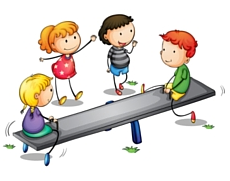
\includegraphics[height=0.7cm]{figs/stagesofplay/onlooker} {Onlooker play}
%        \item 
\includegraphics[height=0.7cm]{figs/stagesofplay/parallel}{Parallel play}
%        \item 
\includegraphics[height=0.7cm]{figs/stagesofplay/associative}{Associative play}
%        \item 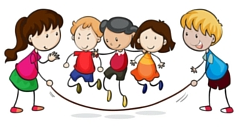
\includegraphics[height=0.7cm]{figs/stagesofplay/cooperative}{Cooperative play}
%    \end{enumerate}
%
%\end{frame}



%%%%%%%%%%%%%%%%%%%%%%%%%%%%%%%%%%%%%%%%%%%%%%%%%%%%%%%%%
%
%\section{Sketching a model}
%
%%%%%%%%%%%%%%%%%%%%%%%%%%%%%%%%%%%%%%%%%%%%%%%%%%%%%%%%%
%
%\begin{frame}{A model of artificial social cognition}
%
%    I postulate {\bf two stages}:
%
%    \begin{enumerate}
%        \item building models of others' minds
%        \item exploiting these models to socially act:
%            \begin{itemize}
%                \item prediction, reading others' intentions
%                \item adapting own behaviour, alignment
%                \item establish join goals
%                \item ultimately, performing joint actions
%            \end{itemize}
%    \end{enumerate}
%
%    \vspace{2em}
%    $\rightarrow$ Social analogs of \emph{perception} \& \emph{action}
%
%\end{frame}
%
%%%%%%%%%%%%%%%%%%%%%%%%%%%%%%%%%%%%%%%%%%%%%%%%%%%%%%%%%
%
%{
%    \paper{see discussion in Vernon, {\bf Artificial Cognitive Systems: A Primer} 2014}
%\begin{frame}{Cognitivist vs Emergent paradigms}
%
%    ``building'', ``exploiting'', ``reading'', ``establishing''... my terminolgy
%    denotes a cognitivist approach (`I, the designer of the system, explicitly implement
%    these capabilities')
%
%    \pause
%    
%    Possible `emergent paradigm' rephrasing:
%
%    \begin{enumerate}
%        \item developing internal states \emph{connoting} others' minds
%        \item perturbing (influencing) actions synthesis with these states
%    \end{enumerate}
%
%    \pause
%
%    {\bf Hybrid approaches} are possible -- mapping to ``raw phenomenal experience'' vs
%    ``access counciousness''.
%\end{frame}
%}
%
%%%%%%%%%%%%%%%%%%%%%%%%%%%%%%%%%%%%%%%%%%%%%%%%%%%%%%%%%
%
%{
%    \paper{Graziano {\bf Consciousness and the Social Brain} -- 2013}
%\begin{frame}[label=attentionschemata]{Modeling others' mind?}
%    \large
%    In cognitive neurosciences: Graziano's \emph{Attention Schemata Theory}
%
%    \begin{columns}
%
%        \begin{column}{0.5\linewidth}
%
%            \begin{center}
%                \includegraphics<1>[width=1.3\columnwidth]{playing_together}
%                \includegraphics<2>[width=1.3\columnwidth]{playing_together_gaze}
%                \includegraphics<3>[width=1.3\columnwidth]{playing_together_awareness}
%                \includegraphics<4>[width=1.3\columnwidth]{playing_together_mutual_awareness}
%            \end{center}
%
%        \end{column}
%
%        \begin{column}{0.5\linewidth}
%
%            \only<2>{
%                \vspace*{1.5cm}
%                Attention is more about {\bf representation} than visual perspective
%
%                \vspace{0.7cm}
%                ``Awareness is a construct that represents the attentional state
%                of a brain''
%
%            }
%            \only<3>{
%                \vspace*{1.5cm}
%                Graziano's postulate that modelling other's state of awareness
%                is {\bf mediated by one's own attentional system}, through joint
%                attention
%            }
%            \only<4>{
%                \vspace*{1.5cm}
%                    It follows that {\bf joint attention is the process that gives
%                    rise to social awareness}
%            }
%
%        \end{column}
%
%    \end{columns}
%
%\end{frame}
%}
%
%%%%%%%%%%%%%%%%%%%%%%%%%%%%%%%%%%%%%%%%%%%%%%%%%%%%%%%%%
%
%\begin{frame}{Sketching a path forward: mentalizing}
%
%    {\bf Hypothesis 1}: Graziano is right: mental representations are snapshots of
%    \emph{awareness}, \emph{awareness} being itself a label for the
%    \emph{memory-mediated process of attention}.
%
%    \pause
%
%    {\bf Hypothesis 2}: this can be extended to social cognition. \textbf{Modeling one
%    other mental representations equates to taking snapshots of their current
%    state of awareness}.
%
%    As we do not have direct access to others' process of attention, it has to
%    be mediated. Following Graziano, we hypotesise that \textbf{modelling other's
%    state of awareness is mediated by one's own attentional system, through
%    joint attention mechanisms}.
%
%
%\end{frame}
%
%
%%%%%%%%%%%%%%%%%%%%%%%%%%%%%%%%%%%%%%%%%%%%%%%%%%%%%%%%
%%%%%%%%%%%%%%%%%%%%%%%%%%%%%%%%%%%%%%%%%%%%%%%%%%%%%%%%%

%\begin{frame}{What does that mean for CRI \& learning?}
%
%    \begin{columns}
%        \begin{column}{0.4\linewidth}
%            
%            \begin{center}
%                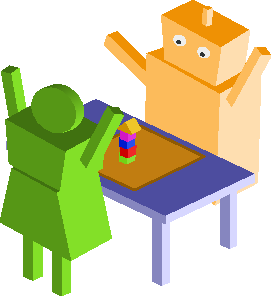
\includegraphics[width=0.9\linewidth]{joint-action-scenario-completed}
%            \end{center}
%        \end{column}
%        \begin{column}{0.6\linewidth}
%            \only<1-4> {
%            \begin{itemize}
%                \item<+-> We can reduce the socio-cognitive cost of
%                    collaboration by relying as much
%                    as possible on {\bf implicit (sub-conscious) social mechanisms}
%                \item<+-> (do not be scared of ambiguous/partially defined
%                    instructions/situations)
%                \item<+-> The robot needs to learn to recognise and interpret
%                    those social cues, hidden within complex social dynamics (in
%                    real-time!)
%                \item<+-> We have some raw material. Time to
%                    process it together!
%            \end{itemize}
%        }
%%            \only<5-> {
%%            \begin{itemize}
%%                \item<+-> Yet, {\bf learning does require cognitive effort \&
%%                    engagement}. We simply want to direct it to the right
%%                    subject.
%%            \end{itemize}
%%        }
%%
%        \end{column}
%    \end{columns}
%\end{frame}

\begin{frame}{In conclusion}

    \begin{columns}
        \begin{column}{0.4\linewidth}
            
            \begin{center}
                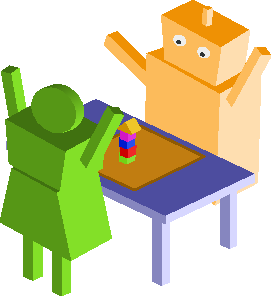
\includegraphics[width=0.9\linewidth]{joint-action-scenario-completed}
            \end{center}
        \end{column}
        \begin{column}{0.6\linewidth}
    \begin{itemize}
        \item<+-> Not only 'child-robot interaction for learning', but also
            'classroom-robot interaction': importance of orchestration
        \item<+-> Right balance \emph{tool}-\emph{social robot}?
        \item<+-> Role of the teacher? \emph{Supervised autonomy} looks like a
            possible direction.
        \item<+-> \emph{Doing together} with the child will require a better
            understanding of the social dynamics. Machine learning to the
            rescue?
    \end{itemize}
        \end{column}
    \end{columns}
\end{frame}

%
%{
%    \fullbackground[color=white]{c-r-t-succeed-dim}
%\begin{frame}[plain]
%
%    {\Large Two open questions for the aspiring PhDs:}
%
%    \begin{itemize}
%        \item<+-> What about group dynamics?
%        \item<+-> Over time, what place would a social robot take in the
%            classroom?
%    \end{itemize}
%\end{frame}
%}
%

{
    \fullbackground[color=white]{c-r-t-succeed}
\begin{frame}[plain]

    \begin{columns}
        \begin{column}{0.5\linewidth}
        \vspace{4cm}

        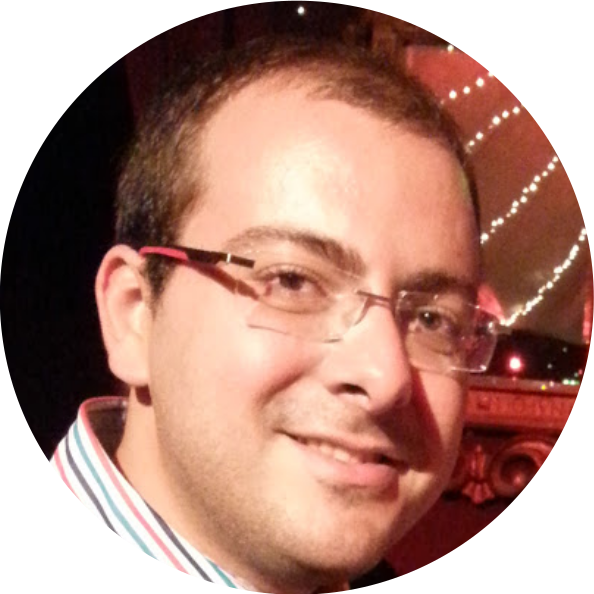
\includegraphics[width=0.3\linewidth]{ayberk}
        \hspace{0.1cm}
        
\includegraphics[width=0.3\linewidth]{deana}

        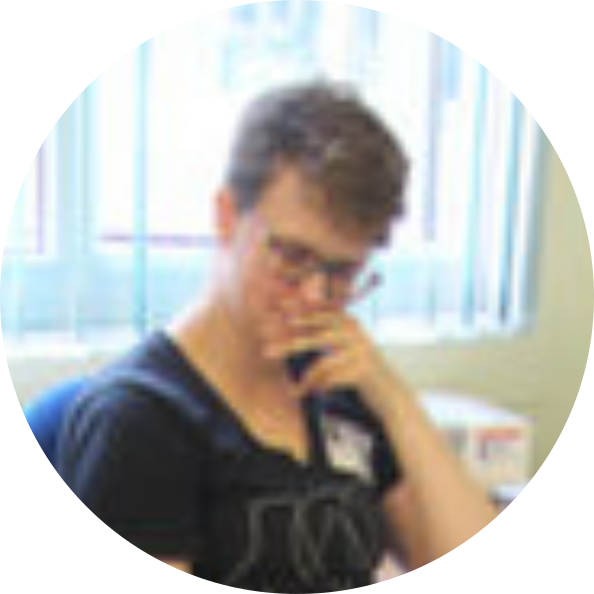
\includegraphics[width=0.3\linewidth]{charlotte}
        \hspace{0.1cm}
        
\includegraphics[width=0.3\linewidth]{emmanuel}

        
\includegraphics[width=0.3\linewidth]{chris}
        \hspace{0.1cm}
        
\includegraphics[width=0.3\linewidth]{maddy}

        \end{column}
        \begin{column}{0.5\linewidth}

    \vspace{6cm}
\setbeamercolor{hriSec1Demo}{fg=white!30!black}
\begin{beamercolorbox}[wd=\linewidth,ht=6ex,dp=0.7ex]{hriSec1Demo}
    \textbf{Thank you!}

\end{beamercolorbox}
        \end{column}
    \end{columns}
\end{frame}
}


%%%%%%%%%%%%%%%%%%%%%%%%%%%%%%%%%%%%%%
\miniframesoff
\section[]{Some more stuff}
\begin{frame}{Some building blocks exists}

    \begin{itemize}
        \item \textbf{Multi-modal fusion}

            \begin{itemize}
                \item \eg Noda et al. {\bf Multimodal integration learning of robot behavior
    using DNN}, Robotics and Autonomous Systems 2014
            \end{itemize}

        \item \textbf{Behavioural sequences recognition}
            \begin{itemize}
                \item How et al. {\bf Behavior recognition for humanoid
                    robots using long short-term memory},
                    IJARS 2016 \emph{$\rightarrow$ LSTM to recognise Nao
                    behaviours}
                \item Shiarlis et al. {\bf Acquiring Social Interaction
                    Behaviours for Telepresence Robots via Deep Learning from
                    Demonstration}, IROS 2017
            \end{itemize}
    \end{itemize}

    \pause
    {\bf DBSoC: Deep Behavioural Social Cloning} -- LfD + CNNs + LSTM

    Two tasks for a telepresence robot:
    \begin{enumerate}
        \item position itself in a (dynamic) group of persons
        \item follow 2 persons
    \end{enumerate}
\end{frame}

{
    \paper{taken from a NIPS2015 tutorial by Geoff Hinton, Yoshua Bengio \&
    Yann LeCun}

\begin{frame}{Deep networks $\equiv$ black boxes?}

    \begin{center}
        \includegraphics<1>[width=\linewidth]{cnn-features}
        \includegraphics<2>[width=0.55\linewidth]{cnn-hi-level-features}
    \end{center}
\end{frame}
}

{
    \paper{Lemaignan et al. {\bf Learning by Teaching a Robot: The Case of Handwriting} -- Robotics and Automation Magazine 2016}
\begin{frame}{Learning to draw a 5}
    \begin{center}
        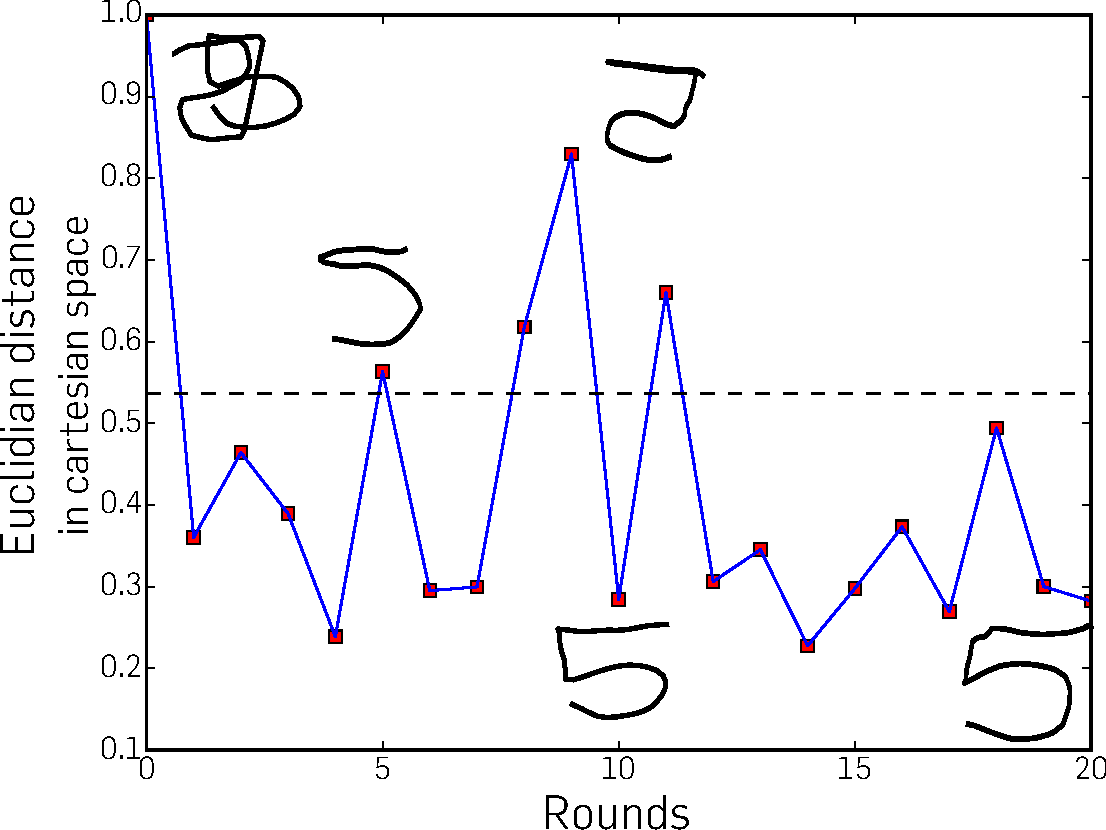
\includegraphics[width=0.8\linewidth]{cowriter/henry5}
    \end{center}
    \badge{epfl}
\end{frame}
}


{
    \paper{Hood, Lemaignan et al. {\bf When Children Teach a Robot to Write: An
    Autonomous Teachable Humanoid [...]} -- HRI 2015}
\begin{frame}{CoWriter implementation}
    \centering

    \only<1>{
        \video{0.9\textwidth}{figs/cowriter/nao-tablet-demo.mp4}
    }

    \only<2>{
        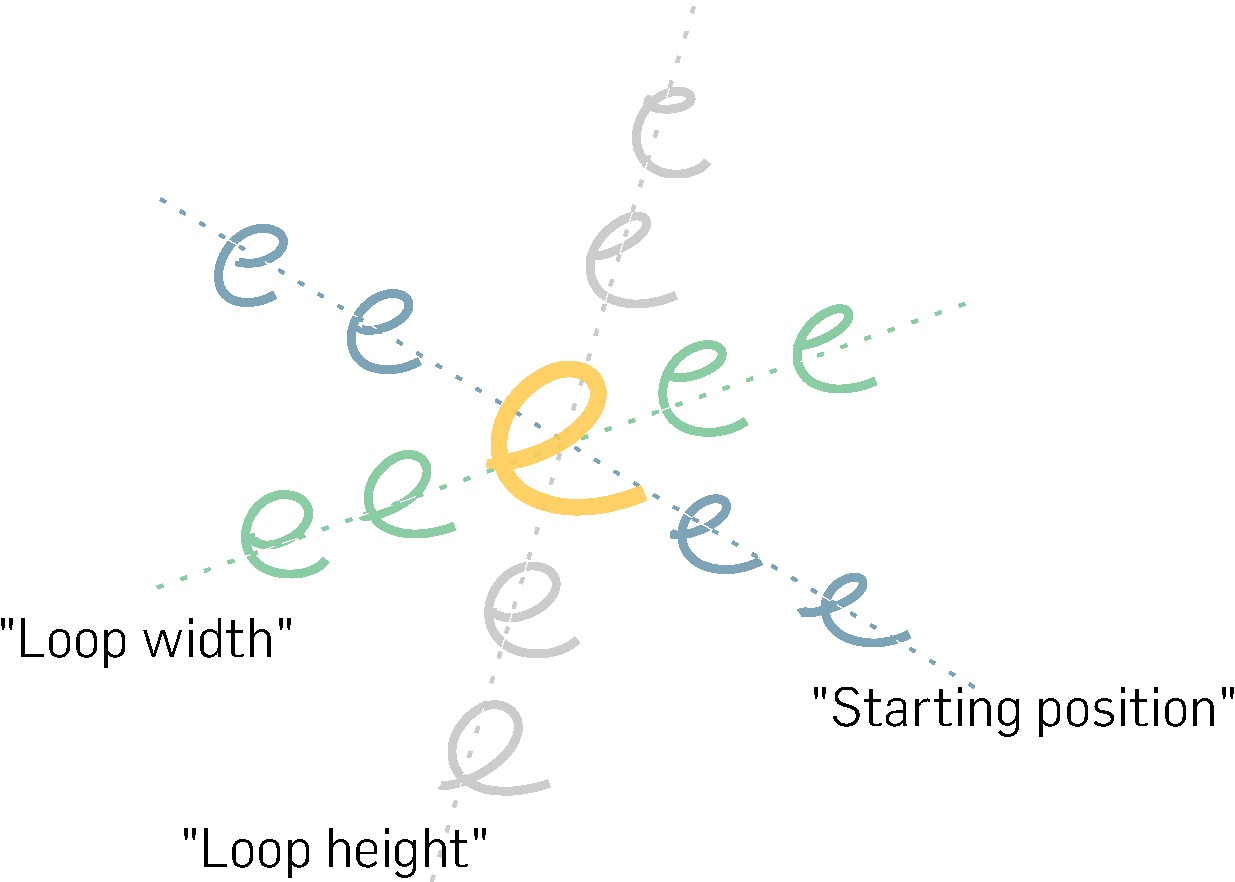
\includegraphics[width=0.8\textwidth]{cowriter/pca}
    }

    \only<3>{
        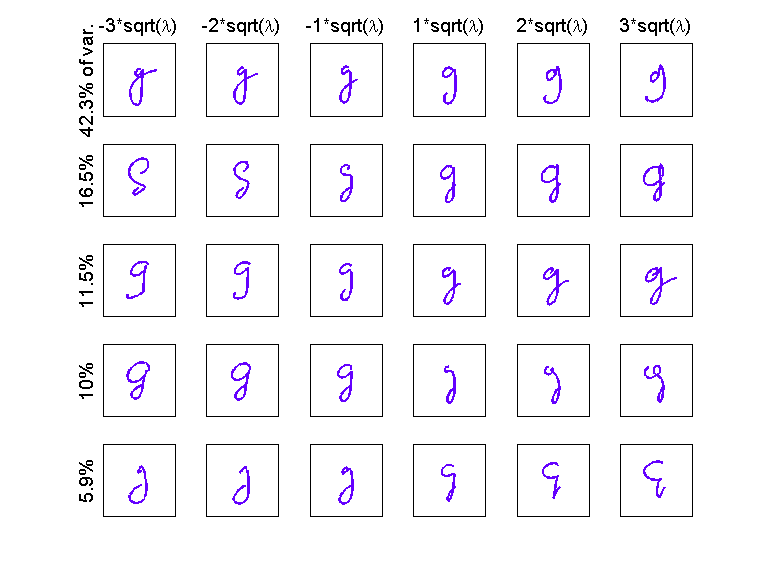
\includegraphics[width=0.8\textwidth]{cowriter/cowriter-g.png}
    }

    \only<4>{
        
\includegraphics[width=0.8\textwidth]{cowriter/learningSdemo}
    }

    %\badge{epfl}
    \badge{deana-epfl}
\end{frame}
}

%%%%%%%%%%%%%%%%%%%%%%%%%%%%%%%%%%%%%%%%%%%%%%%%%%%%%%%%

\begin{frame}[plain]
    \begin{center}
        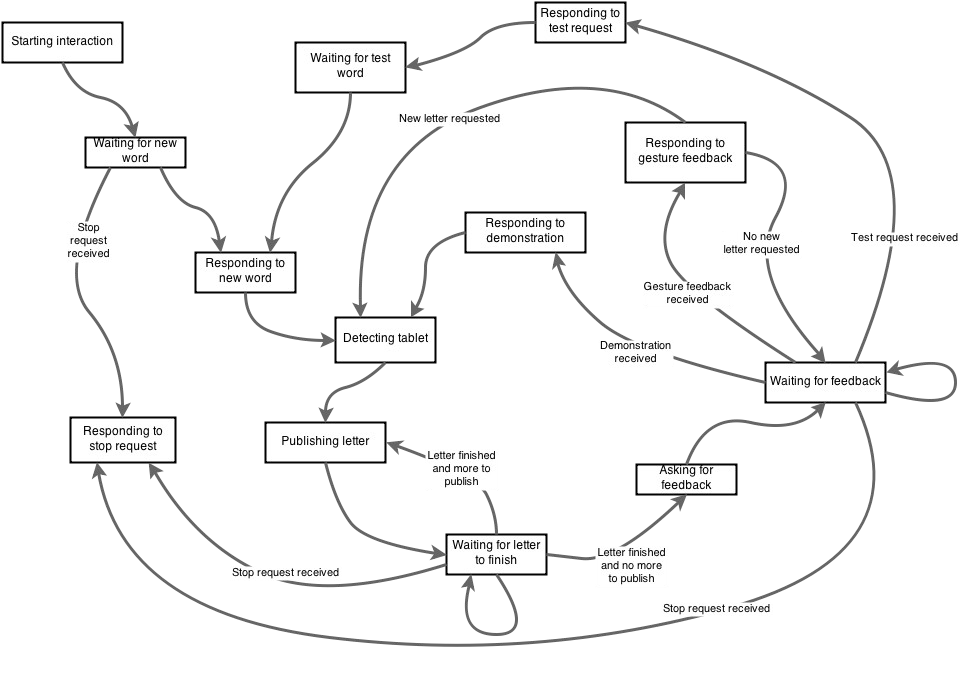
\includegraphics[width=0.8\linewidth]{cowriter/cowriter-fsm.png}
    \end{center}

    \backbutton{}
\end{frame}


{
    \paper{Hostettler, \"Ozg\"ur, Lemaignan et al. {\bf Real-Time High-Accuracy
    2D Localization with Structured Patterns} -- ICRA 2016}
 \begin{frame}{Interaction with the paper}
     \badge{ayberk-epfl}
     Critically, Cellulo is meant as an {\bf interaction between
     (classroom-friendly) paper and the robots}.

     \pause

     Achieved through a {\bf paper-based absolute localisation system}

     \begin{center}
         \includegraphics<3>[width=0.8\linewidth]{cellulo/treasure-game-1}
         \includegraphics<4>[width=\linewidth]{cellulo/treasure-game-2}
     \end{center}

     \only<5>{

         \begin{itemize}
             \item even more than 'classroom-friendly', paper is 'teacher-friendly'
             \item easy to manipulate, copy, print, cutout, dispose...
             \item unique activity IDs: drop the robots onto the sheet, it
                 recognizes the activity
         \end{itemize}
     }

 \end{frame}
}

\imageframe[caption={Learning-related game actions}, scale=0.9]{sparc/d_eat}

\begin{frame}{What did we record?}

\small
\begin{tabular}{@{}lll@{}}
\toprule
\textbf{Domain} & \textbf{Type}                              & \textbf{Details}                          \\ \midrule
child $\times$ 2        & audio                                      & 16kHz, mono, semi-directional             \\
                & face (RGB)                                 & qHD (960x540), 30Hz                       \\
                & face (depth)                               & VGA (640x480), 30Hz                       \\
                & facial features                            & 70 2D points, 30Hz                        \\
                & skeleton                                   & 15 2D points, 30Hz                        \\
                & hands                                      & 20 x 2 2D points, 30Hz                    \\ \midrule
environment     & RGB                                        & qHD (960x540), 29.7Hz                     \\ \midrule
touchscreen     & background drawing (RGB)                   & 4Hz                                       \\
                & touches                                    & 6 points multi-touch, 10Hz                \\
                & items position and orientation             & (x,y,theta), 10Hz                         \\ \midrule
annotations     & \multicolumn{2}{l}{timestamped annotations of social behaviours} \\\midrule
+ post-process          & \multicolumn{2}{l}{optical flow, audio features}           \\
                & \multicolumn{2}{l}{facial action units...}                                   \\ \bottomrule
\end{tabular}

\end{frame}

\end{document}
